\documentclass[a4paper]{arrowhead}

\usepackage[yyyymmdd]{datetime}
\usepackage{etoolbox}
\usepackage[utf8]{inputenc}
\usepackage[T1]{fontenc}
\usepackage{multirow}
\usepackage{longtable}
\usepackage{array}
\newcolumntype{P}[1]{>{\raggedright\arraybackslash}p{#1}}
\newcolumntype{Y}{>{\raggedright\arraybackslash}X}
\usepackage{enumitem}
\usepackage{tikz}
\usepackage{adjustbox}
\usepackage{placeins}
\BeforeBeginEnvironment{tikzpicture}{\begin{adjustbox}{max width=\textwidth}}
\AfterEndEnvironment{tikzpicture}{\end{adjustbox}}
\usepackage{xurl}
\usetikzlibrary{arrows.meta,positioning,shapes.geometric,fit,calc,backgrounds}

\renewcommand{\dateseparator}{-}
\setlist{itemsep=1pt,topsep=3pt}


% Keep long identifiers readable in narrow table columns.
\ExplSyntaxOn
\NewDocumentCommand{\ahbreak}{m}{
  \tl_set:Nn \l_tmpa_tl {#1}
  \regex_replace_all:nnN {([a-z])([A-Z])} {\1\c{allowbreak}\2} \l_tmpa_tl
  \tl_use:N \l_tmpa_tl
}
\ExplSyntaxOff

%% Identifier styles
\newcommand{\sys}[1]{\textcolor{ArrowheadBlue}{\textbf{\ahbreak{#1}}}}      % microsystem
\newcommand{\svc}[1]{\textcolor{ArrowheadPurple}{\textit{\ahbreak{#1}}}}    % microservice (service definition)
\newcommand{\op}[1]{\prop{#1}}                                  % service operation
\makeatletter\g@addto@macro\UrlBreaks{\do\.\do\_\do\-\do\,\do\|}\makeatother
\DeclareUrlCommand\prop{\urlstyle{tt}}                             % configuration property / code identifier

%% TikZ styles
\tikzset{
  sysbox/.style={draw=ArrowheadBlue, very thick, fill=white, rounded corners=2pt,
                 minimum width=3.6cm, minimum height=1.0cm, align=center, font=\small\bfseries},
  supbox/.style={draw=ArrowheadTeal, thick, dashed, fill=AHSysMLSupport, rounded corners=2pt,
                 minimum width=3.2cm, minimum height=0.9cm, align=center, font=\small},
  appbox/.style={draw=ArrowheadGrey, thick, fill=AHSysMLApplication, rounded corners=2pt,
                 minimum width=3.2cm, minimum height=0.9cm, align=center, font=\small},
  layer/.style={draw=ArrowheadGrey, fill=white, minimum width=11.6cm, text width=11.2cm, minimum height=0.75cm,
                align=center, font=\small},
  flt/.style={draw=ArrowheadOrange, thick, fill=white, rounded corners=2pt,
              minimum width=2.8cm, minimum height=1.1cm, align=center, font=\scriptsize},
  pstep/.style={draw=ArrowheadBlue, fill=white, rounded corners=2pt, minimum width=7.4cm,
               minimum height=0.55cm, align=left, font=\scriptsize, text width=7.2cm},
  cond/.style={draw=ArrowheadOrange, fill=white, rounded corners=2pt,
               align=left, font=\scriptsize, text width=4.8cm},
  uses/.style={-{Stealth[length=2.2mm]}, thick, ArrowheadGrey},
  opt/.style={-{Stealth[length=2.2mm]}, thick, dashed, ArrowheadTeal},
  msg/.style={-{Stealth[length=2mm]}, thick},
  ret/.style={-{Stealth[length=2mm]}, dashed},
  lifeline/.style={densely dashed, gray},
  head/.style={draw=ArrowheadBlue, fill=white, thick, minimum width=2.5cm,
               minimum height=0.7cm, align=center, font=\scriptsize\bfseries},
  ahead/.style={draw=ArrowheadGrey, fill=AHSysMLApplication, thick, minimum width=2.5cm,
               minimum height=0.7cm, align=center, font=\scriptsize\bfseries},
  lbl/.style={font=\scriptsize, fill=white, inner sep=1pt},
  num/.style={circle, fill=ArrowheadBlue, text=white, font=\tiny\bfseries, inner sep=1pt, minimum size=3.4mm}
}

%% Sequence-diagram helpers: \lifelines{list of x:name:style}{depth}
\newcommand{\seqhead}[4]{\node[#4] at (#2,0) {#3}; \draw[lifeline] (#2,-0.6) -- (#2,-#1);}

% Exact RGB fills decoded from Papyrus notation packed BGR integers.
% Source: profile-library-sysml/distribution/SysML-v1.6/Papyrus/
% ArrowheadDSL_2025_v5/SysML v1.6/EclipseArrowhead-5.0/Arrowhead-5.0.notation
% ServiceRegistry 16750080; security 9983; combined-cloud orchestration 63744.
% Earlier standalone orchestration views also use 7928434 (72FA78).
\definecolor{AHSysMLRegistry}{HTML}{0096FF}
\definecolor{AHSysMLSecurity}{HTML}{FF2600}
\definecolor{AHSysMLOrchestration}{HTML}{00F900}
\definecolor{AHSysMLSupport}{HTML}{FEFB00}
\definecolor{AHSysMLApplication}{HTML}{FF9300}
\definecolor{AHSysMLInterface}{HTML}{9BC7CC}
\definecolor{AHSysMLInfrastructure}{HTML}{C0C0C0}
% Aliases keep existing black-box diagrams on the same exact palette.
\colorlet{SRBlue}{AHSysMLRegistry}
\colorlet{AuthzRed}{AHSysMLSecurity}
\colorlet{AuthnLilac}{AHSysMLSecurity}
\colorlet{OrchGreen}{AHSysMLOrchestration}
\colorlet{AppOrange}{AHSysMLApplication}
\colorlet{SupTeal}{AHSysMLSupport}
\tikzset{
 ahRegistry/.style={fill=AHSysMLRegistry,draw=black!80,text=black},
 ahAuthentication/.style={fill=AHSysMLSecurity,draw=black!80,text=black},
 ahAuthorization/.style={fill=AHSysMLSecurity,draw=black!80,text=black},
 ahOrchestration/.style={fill=AHSysMLOrchestration,draw=black!80,text=black},
 ahSupport/.style={fill=AHSysMLSupport,draw=black!80,text=black},
 ahApplication/.style={fill=AHSysMLApplication,draw=black!80,text=black},
 ahInterface/.style={fill=AHSysMLInterface,draw=black!80,text=black},
 ahInfrastructure/.style={fill=AHSysMLInfrastructure,draw=black!80,text=black},
 lolli/.append style={fill=AHSysMLInterface,draw=black!80},
 ahMixed/.style={fill=white,draw=black!65,text=black}
}


\begin{document}

%% Arrowhead Document Properties
\ArrowheadTitle{Arrowhead Core Systems 5.3.0 -- White Box}
\ArrowheadType{Generic System of Systems Design Description}
\ArrowheadTypeShort{GSoSDD}
\ArrowheadVersion{5.3.0}
\ArrowheadDate{2026-11-03}
\ArrowheadAuthor{Jerker Delsing}
\ArrowheadStatus{DRAFT}
\ArrowheadContact{jerker.delsing@ltu.se}
\ArrowheadFooter{\href{https://www.arrowhead.eu}{www.arrowhead.eu}}
\ArrowheadSetup
%%

%% Front Page
\begin{center}
  \vspace*{1cm}
  \huge{\arrowtitle}

  \vspace*{0.2cm}
  \LARGE{\arrowtype}
  \vspace*{1cm}

  \vspace*{\fill}

  \begin{tikzpicture}[node distance=0.6cm and 0.7cm, scale=0.85, every node/.style={transform shape}]
    \node[sysbox, ahRegistry] (sr) {ServiceRegistry};
    \node[sysbox, above left=0.9cm and 0.5cm of sr, ahAuthentication] (auth) {Authentication};
    \node[sysbox, above right=0.9cm and 0.5cm of sr, ahAuthorization] (ca) {ConsumerAuthorization};
    \node[sysbox, below left=0.9cm and 0.5cm of sr, ahOrchestration] (dso) {DynamicService-\\Orchestration};
    \node[sysbox, below right=0.9cm and 0.5cm of sr, ahOrchestration] (sso) {SimpleStoreService-\\Orchestration};
    \foreach \n in {auth,ca,dso,sso} \draw[uses] (\n) -- (sr);
  \end{tikzpicture}

  \vspace*{1cm}
  \vspace*{\fill}

  \begin{abstract}
    This document is the white-box Generic System of Systems Design Description (GSoSDD) of the
    Eclipse Arrowhead 5 Core Systems as release candidate version 5.3.0. It complements the
    black-box, technology-agnostic \emph{GSoSD Arrowhead Core and Support Systems 5.3.0}
    \cite{gsosd522} (successor of \emph{GSoSD Arrowhead Core Systems 5.0} \cite{gsosd50}) by
    describing how the five released Core microsystems -- \sys{ServiceRegistry},
    \sys{Authentication}, \sys{ConsumerAuthorization}, \sys{DynamicServiceOrchestration} and
    \sys{SimpleStoreServiceOrchestration} -- are actually designed, configured and interconnected
    in the reference implementation (\prop{ah5-core-java-spring} v5.2.2 on
    \prop{ah5-common-java-spring} 5.2.2), including their internal processing chains, data
    stores, produced and consumed services, security mechanisms, and the optional
    interaction with the 5.2.2 Support Systems \sys{Blacklist}, \sys{TranslationManager} and
    \sys{DeviceQoSEvaluator}.
  \end{abstract}

  \vspace*{1cm}
\end{center}

\newpage
%%

\tableofcontents
\newpage

%% ============================================================================================
\section{Overview}
\label{sec:overview}

This SoSDD white box document provides the foundational Eclipse
Arrowhead framework core system reference implementation
specifications enabling the creation of technology and engineering platforms for any application domain solution.

\paragraph{Graphics colour convention.}
All diagrams registry blue, authentication
and authorization red-orange, orchestration green, support yellow and application
orange. Both orchestration implementations share 
green; infrastructure is grey and mixed-system groups are neutral. These colours
identify roles rather than implementation languages. Turquoise is
reserved for service-interface elements. The SysML v1.6 Papyrus
library's system-role fills, taken from \prop{EclipseArrowhead-5.0/Arrowhead-5.0.notation} provides further
color details.
\begin{center}\scriptsize
\setlength{\fboxsep}{4pt}
\colorbox{AHSysMLRegistry}{\strut ServiceRegistry}\quad
\colorbox{AHSysMLSecurity}{\strut Authentication / ConsumerAuthorization}\\[6pt]
\colorbox{AHSysMLOrchestration}{\strut DSO / SimpleStore orchestration}\quad
\colorbox{AHSysMLSupport}{\strut Support}\quad
\colorbox{AHSysMLApplication}{\strut Application}\quad
\colorbox{AHSysMLInfrastructure}{\strut Infrastructure}
\end{center}

%\paragraph{Graphics colour convention.}
All diagrams use the SysML v1.6 Papyrus library's system-role fills, taken from
\prop{EclipseArrowhead-5.0/Arrowhead-5.0.notation}: registry blue, authentication
and authorisation red-orange, orchestration green, support yellow and application
orange. Both orchestration implementations share the library's combined-cloud
green; infrastructure is grey and mixed-system groups are neutral. These colours
identify roles rather than implementation languages. The library's turquoise is
reserved for service-interface elements.
\begin{center}\scriptsize
\setlength{\fboxsep}{4pt}
\colorbox{AHSysMLRegistry}{\strut ServiceRegistry}\quad
\colorbox{AHSysMLSecurity}{\strut Authentication / ConsumerAuthorization}\\[6pt]
\colorbox{AHSysMLOrchestration}{\strut DSO / SimpleStore orchestration}\quad
\colorbox{AHSysMLSupport}{\strut Support}\quad
\colorbox{AHSysMLApplication}{\strut Application}\quad
\colorbox{AHSysMLInfrastructure}{\strut Infrastructure}
\end{center}


% \subsection{Implementation baseline and roadmap status (30 October 2026)}
% \label{sec:baseline-20261030}
% The architecture is realised by three primary source distributions:
% \prop{Eclipse-Arrowhead-java}, \prop{Eclipse-Arrowhead-go} and
% \prop{Eclipse-Arrowhead-rust}, under the Eclipse workspace. These are the
% sources for subsequent implementation changes; older \prop{Arrowhead/} and
% \prop{EA-fork/} checkouts are historical references or deployment consumers.
% A primary-source designation does not imply that every running image has been
% rebuilt from that tree. Release v5.2.2, local extensions, independently packaged
% sources and dated deployment evidence remain distinct \cite{primaryBaseline20261030}.

% \begin{table}[htbp]
% \centering\small
% \begin{tabularx}{\textwidth}{|P{1.6cm}|X|X|}\hline
% \rowcolor{gray!20} Language & Current source/build boundary & Evidence and limits \\\hline
% Java & Five core systems in \prop{ah5-core-java-spring}; fifteen independent
% support projects with own JAR/image/configuration. The Java-cloud manager is
% Node.js/nginx, despite its folder name. & Support packaging verified on
% 25 October; core/support services and operations tools have separate lifecycles.
% No shared JavaSupportRuntime dependency in the fifteen standalone projects. \\\hline
% Go & Five independent core modules and eighteen current top-level support/test/tool
% modules; private helper copies and optional \prop{go.work}. & 28 October audit:
% 22 module builds, tests and vet checks passed. Packaging does not establish
% complete Java parity or a new live rollout. \\\hline
% Rust & Five core entry points; fifteen support entry points and a separate
% LocalCloudManager crate in one Cargo workspace. Core/support libraries and
% messaging remain shared build dependencies. & 28 October copy report:
% 147 workspace tests passed. Per-system folders are not independently copied
% source closures. Java-equivalence and operational qualification remain open. \\\hline
% \end{tabularx}
% \caption{Current implementation structure, not a language-equivalence claim.
% Dated evidence is retained in each primary distribution
% \cite{javaPackaging20261025,goPackaging20261028,rustPackaging20261028}.}
% \end{table}
% \FloatBarrier

% \paragraph{Core inventory versus default cloud.}
% Five core implementations remain available. A \emph{new Java local-cloud design}
% selects ServiceRegistry, Authentication, ConsumerAuthorization and
% DynamicServiceOrchestration. SimpleStoreServiceOrchestration (labelled
% SimpleOrchestration by the configurator) is optional and absent from that default;
% it has not been deleted or implicitly stopped in an existing cloud. This is a
% configuration default, not a removal of the simple-store architecture or a new
% upstream release requirement \cite{javaLocalCloud20261030}.

% \paragraph{Database ownership and access boundary.}
% Every defined database is an \emph{integrated asset of its owning microsystem},
% including a separately deployed SQL or graph-database container. It is not
% selectable shared infrastructure or an independent service provider. Only host
% internal actions or services produced/consumed by that host mediate data access.
% The ownership rule also applies to embedded SQLite and private snapshot files.
% Brokers, relays and the constrained Docker proxy remain infrastructure. The
% Java catalog implements this rule for all sixteen defined database services;
% the default canvas therefore contains four microsystems, each with its own
% database, and one AMQP broker. The database assets do not become extra graph
% nodes \cite{javaDatabaseAssets20261030}.

% \begin{figure}[htbp]
% \centering
% % Current Java default design: owned assets are nested inside host boundaries.
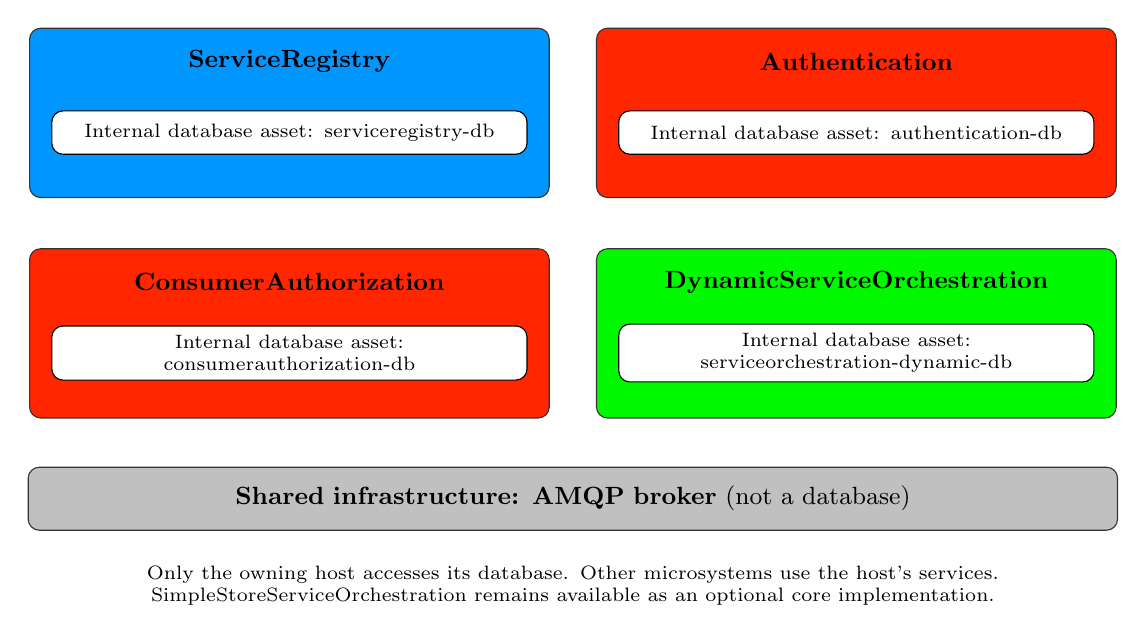
\begin{tikzpicture}[x=1cm,y=1cm,font=\small,
 host/.style={draw,rounded corners,minimum width=6.6cm,minimum height=2.15cm},
 asset/.style={draw,fill=white,rounded corners,text width=5.8cm,align=center,font=\scriptsize,minimum height=0.55cm}]
\node[host,ahRegistry] (sr) at (0,0) {};
\node at (0,0.65) {\textbf{ServiceRegistry}};
\node[asset] at (0,-0.25) {Internal database asset: serviceregistry-db};
\node[host,ahAuthentication] (auth) at (7.2,0) {};
\node at (7.2,0.65) {\textbf{Authentication}};
\node[asset] at (7.2,-0.25) {Internal database asset: authentication-db};
\node[host,ahAuthorization] (ca) at (0,-2.8) {};
\node at (0,-2.15) {\textbf{ConsumerAuthorization}};
\node[asset] at (0,-3.05) {Internal database asset: consumerauthorization-db};
\node[host,ahOrchestration] (dso) at (7.2,-2.8) {};
\node at (7.2,-2.15) {\textbf{DynamicServiceOrchestration}};
\node[asset] at (7.2,-3.05) {Internal database asset: serviceorchestration-dynamic-db};
\node[draw,rounded corners,ahInfrastructure,text width=13.6cm,align=center,minimum height=0.8cm] at (3.6,-4.9)
 {\textbf{Shared infrastructure: AMQP broker} (not a database)};
\node[text width=13.6cm,align=center,font=\scriptsize] at (3.6,-6.0)
 {Only the owning host accesses its database. Other microsystems use the host's services.\\
 SimpleStoreServiceOrchestration remains available as an optional core implementation.};
\end{tikzpicture}

% \caption{New Java default design. Each database is nested inside its owning
% microsystem boundary; it is not shared infrastructure or an independently
% selectable component. Colors retain the established Arrowhead system roles.}
% \label{fig:default-owned-assets}
% \end{figure}
% \FloatBarrier

% \paragraph{Evidence-qualified roadmap.}
% Recorded 19--24 October interoperability and federation results below remain
% historical acceptance of the stated workloads. The 23 October operation-count
% audit has not been replaced by a new complete differential audit. The Go
% packaging audit records a failing optional native-registry integration test:
% orchestration service registration is rejected, including with unmodified
% reference sources. Rust still has partial DTO/error/side-effect coverage,
% unsupported integrations and no automatic Java-state import. Complete
% replacement requires contract, policy, persistence and mixed-cloud acceptance
% for the exact image/configuration, beyond successful packaging tests
% \cite{goPackaging20261028,rustPackaging20261028,nativeCompatibility20261024}.

% \subsection{Core implementation and local-cloud lifecycle updates}
% \label{sec:core-lifecycle-update}
% The detailed Java layers and service contracts below remain the reference design.
% Go modules are separately buildable with \prop{GOWORK=off}; Rust per-system entry
% points call the shared core library. Private Go helper copies require security
% fixes in each affected module; Rust library updates require rebuilding affected
% binaries. Folder symmetry does not mean identical build or persistence models.

% Java core SQL containers and their volumes belong inside each core microsystem's
% white-box boundary. Go/Rust private persistent snapshots are likewise owned
% state, not services shared with other microsystems. Existing Java SQL state and
% sessions are not automatically migrated when substituting a Go/Rust binary.
% The five implementations and their contracts remain documented; selecting the
% four-system default does not remove the simple-store implementation.

% The Java LocalCloudConfigurator catalog groups each host's database and service
% under one owner. A dependency-ordered plan starts the database before its host;
% an explicit host stop reverses that order and retains volumes. Independent
% database stop requests are refused. The executor validates catalog hash, owner,
% step kind and exact target, refuses host startup without its running database,
% and refuses database shutdown while the host is running. Each of the sixteen
% containerised Java-cloud databases has a dedicated internal network shared only
% with its host, with no published database port; all sixteen boundaries were
% checked against Compose and Docker runtime on 30 October
% \cite{javaDatabaseAssets20261030}.

% Plan review and application remain separate: a fresh runtime plan must match the
% reviewed hash, and only one active deployment is accepted across API restarts.
% Core systems, required infrastructure and manager access are protected. The
% private API uses an operator bearer credential through the manager proxy; it
% adds no Arrowhead identity or grants. ColonyOS commands are authenticated and
% catalog checked; operations scripts are not a distributed transaction and have
% no automatic rollback. The host executor uses an immutable content-addressed JAR
% and assignment heartbeats preserve API liveness. The verification report records
% 20 Java tests, ten focused manager/editor tests and ten live browser check
% groups. Live execution verified the baseline without mutating microsystems;
% start/stop paths were unit-tested \cite{javaDatabaseAssets20261030}.



% The Eclipse Arrowhead project provides a SOA/microservice architecture infrastructure that
% enables the creation of automation solutions built from loosely coupled, late-bound microsystems
% which produce and consume microservices from the deep edge to the cloud. The Core microsystems
% manage the complexity introduced by this distribution by providing \emph{discovery},
% \emph{authentication}, \emph{authorisation} and \emph{orchestration} for a local cloud.

% The black-box \emph{GSoSD Arrowhead Core and Support Systems 5.2.2} \cite{gsosd522}, like its
% predecessor \emph{GSoSD Arrowhead Core Systems 5.0} \cite{gsosd50}, describes these concerns in the
% abstract (black box): what problems the Core systems solve and how they interact, without
% endorsing a specific implementation. The present document is its \emph{white-box} counterpart.
% It opens the boxes and describes, for the 5.2.2 release of the reference implementation:

% \begin{itemize}
%   \item which microsystems realise the abstract Core functions and how they are decomposed
%         internally (layers, filter chains, engines, persistent data);
%   \item the exact microservices, operations, interface templates and default endpoints they
%         produce, and which services each of them consumes;
%   \item the run-time interaction patterns (bootstrapping, discovery, authentication,
%         authorisation, dynamic and store-based orchestration) as realised in code;
%   \item the configuration surface which selects between the alternative behaviours foreseen in
%         the GSoSD (e.g.\ atomic vs.\ advanced orchestration, authentication policies,
%         management policies);
%   \item implementation observations relevant to deployers and to the Roadmap WG.
% \end{itemize}

% The original reference descriptions were derived from the tagged \prop{v5.2.2} sources of
% \prop{ah5-core-java-spring} \cite{ah5core}, the 5.2.2 \prop{arrowhead-common} library
% \cite{ah5common}, the v5.2.2 support system repositories
% \cite{ah5blacklist,ah5translation,ah5qos}, and the AITIA implementation documentation
% \cite{ah5docs}, which holds the per-system SysD/SysDD, SD and IDD documents referenced below.
% Local extensions and current packaging/status updates are sourced separately
% in Section~\ref{sec:baseline-20261030}; they are not claims about the upstream tag.

% The rest of this document is organised as follows. Section~\ref{sec:prior_art} references
% prior art, Section~\ref{sec:use} the intended usage, Section~\ref{sec:properties} the SoS
% properties and Section~\ref{sec:delimitations} the delimitations. Section~\ref{sec:architecture}
% describes the SoS architecture and the internal architecture common to all Core microsystems.
% Section~\ref{sec:systems} gives the white-box description of each microsystem.
% Section~\ref{sec:services} lists produced and consumed services. Section~\ref{sec:usecases}
% presents white-box use cases. Section~\ref{sec:planes} discusses control and data planes,
% Section~\ref{sec:security} security, Section~\ref{sec:nfr} non-functional properties,
% Section~\ref{sec:ports} specifies port numbering for local clouds and systems of local clouds,
% and Section~\ref{sec:issues} lists implementation observations and open issues.

% \newpage

\subsection{Significant Prior Art}
\label{sec:prior_art}

\begin{itemize}
  \item \textbf{Arrowhead Framework 4.x (last 4.6.1).} Core systems sharing a common SQL
        database; Service Registry, Authorization and Orchestrator as the mandatory core. The 5.x
        line breaks backwards compatibility deliberately: every 5.x microsystem owns its own data
        store.
  \item \textbf{GSoSD Arrowhead Core Systems 5.0 v1.2} \cite{gsosd50}. Defines the abstract
        Core: Service Registry, Authorisation, Authentication and Orchestration systems, the two
        orchestration approaches (\emph{atomic} and \emph{advanced}), the authorisation priority
        rule (local cloud Authorisation System rules override application-internal rules), active
        and passive systems, and the backwards-compatibility policy.
   \item \textbf{Foundational properties} \cite{FoundationaProperties}
     Arrowhead foundational properties
   \item \textbf{Based on standards} \cite{BasedOnStandards}
     Standards used in the Arrowhead Framework. 
   \item \textbf{Naming convention} \cite{naming2}. Microsystems in PascalCase, microservices
        (service definitions) in camelCase, operations in kebab-case, interface templates in
        snake\_case. The 5.2.2 implementation enforces this through name normalisers and
        validators in \prop{arrowhead-common}.
  \item \textbf{Arrowhead X.509 certificate profile.} Hierarchical certificate chain
        (master~$\rightarrow$ organisation~$\rightarrow$ local cloud~$\rightarrow$
        device/system/operator) used by the \prop{CERTIFICATE} authentication policy.
\end{itemize}

\subsection{How This SoS Is Meant to Be Used}
\label{sec:use}

A 5.3.0 local cloud extend the v5.2.2 and v5.0 default with full AAA
and encrypted communication security:
ServiceRegistry, Authentication and ConsumerAuthorization provide the protected
discovery and AAA foundation. Orchestration strategy and optional Support systems
are selected for the deployment without weakening that security
baseline. Application microsystems (providers and consumers) 
register themselves and their service instances in the \sys{ServiceRegistry}, obtain an
identity either from an X.509 certificate or from the \sys{Authentication} system, and either
look up providers directly or ask an orchestration system which provider instances to consume.
Providers delegate access decisions to \sys{ConsumerAuthorization}. Figure~\ref{fig:component}
shows the SoS as a component diagram; solid arrows denote service consumption between Core
systems, dashed arrows optional consumption of Support systems.

\begin{figure}[h!]
  \centering
  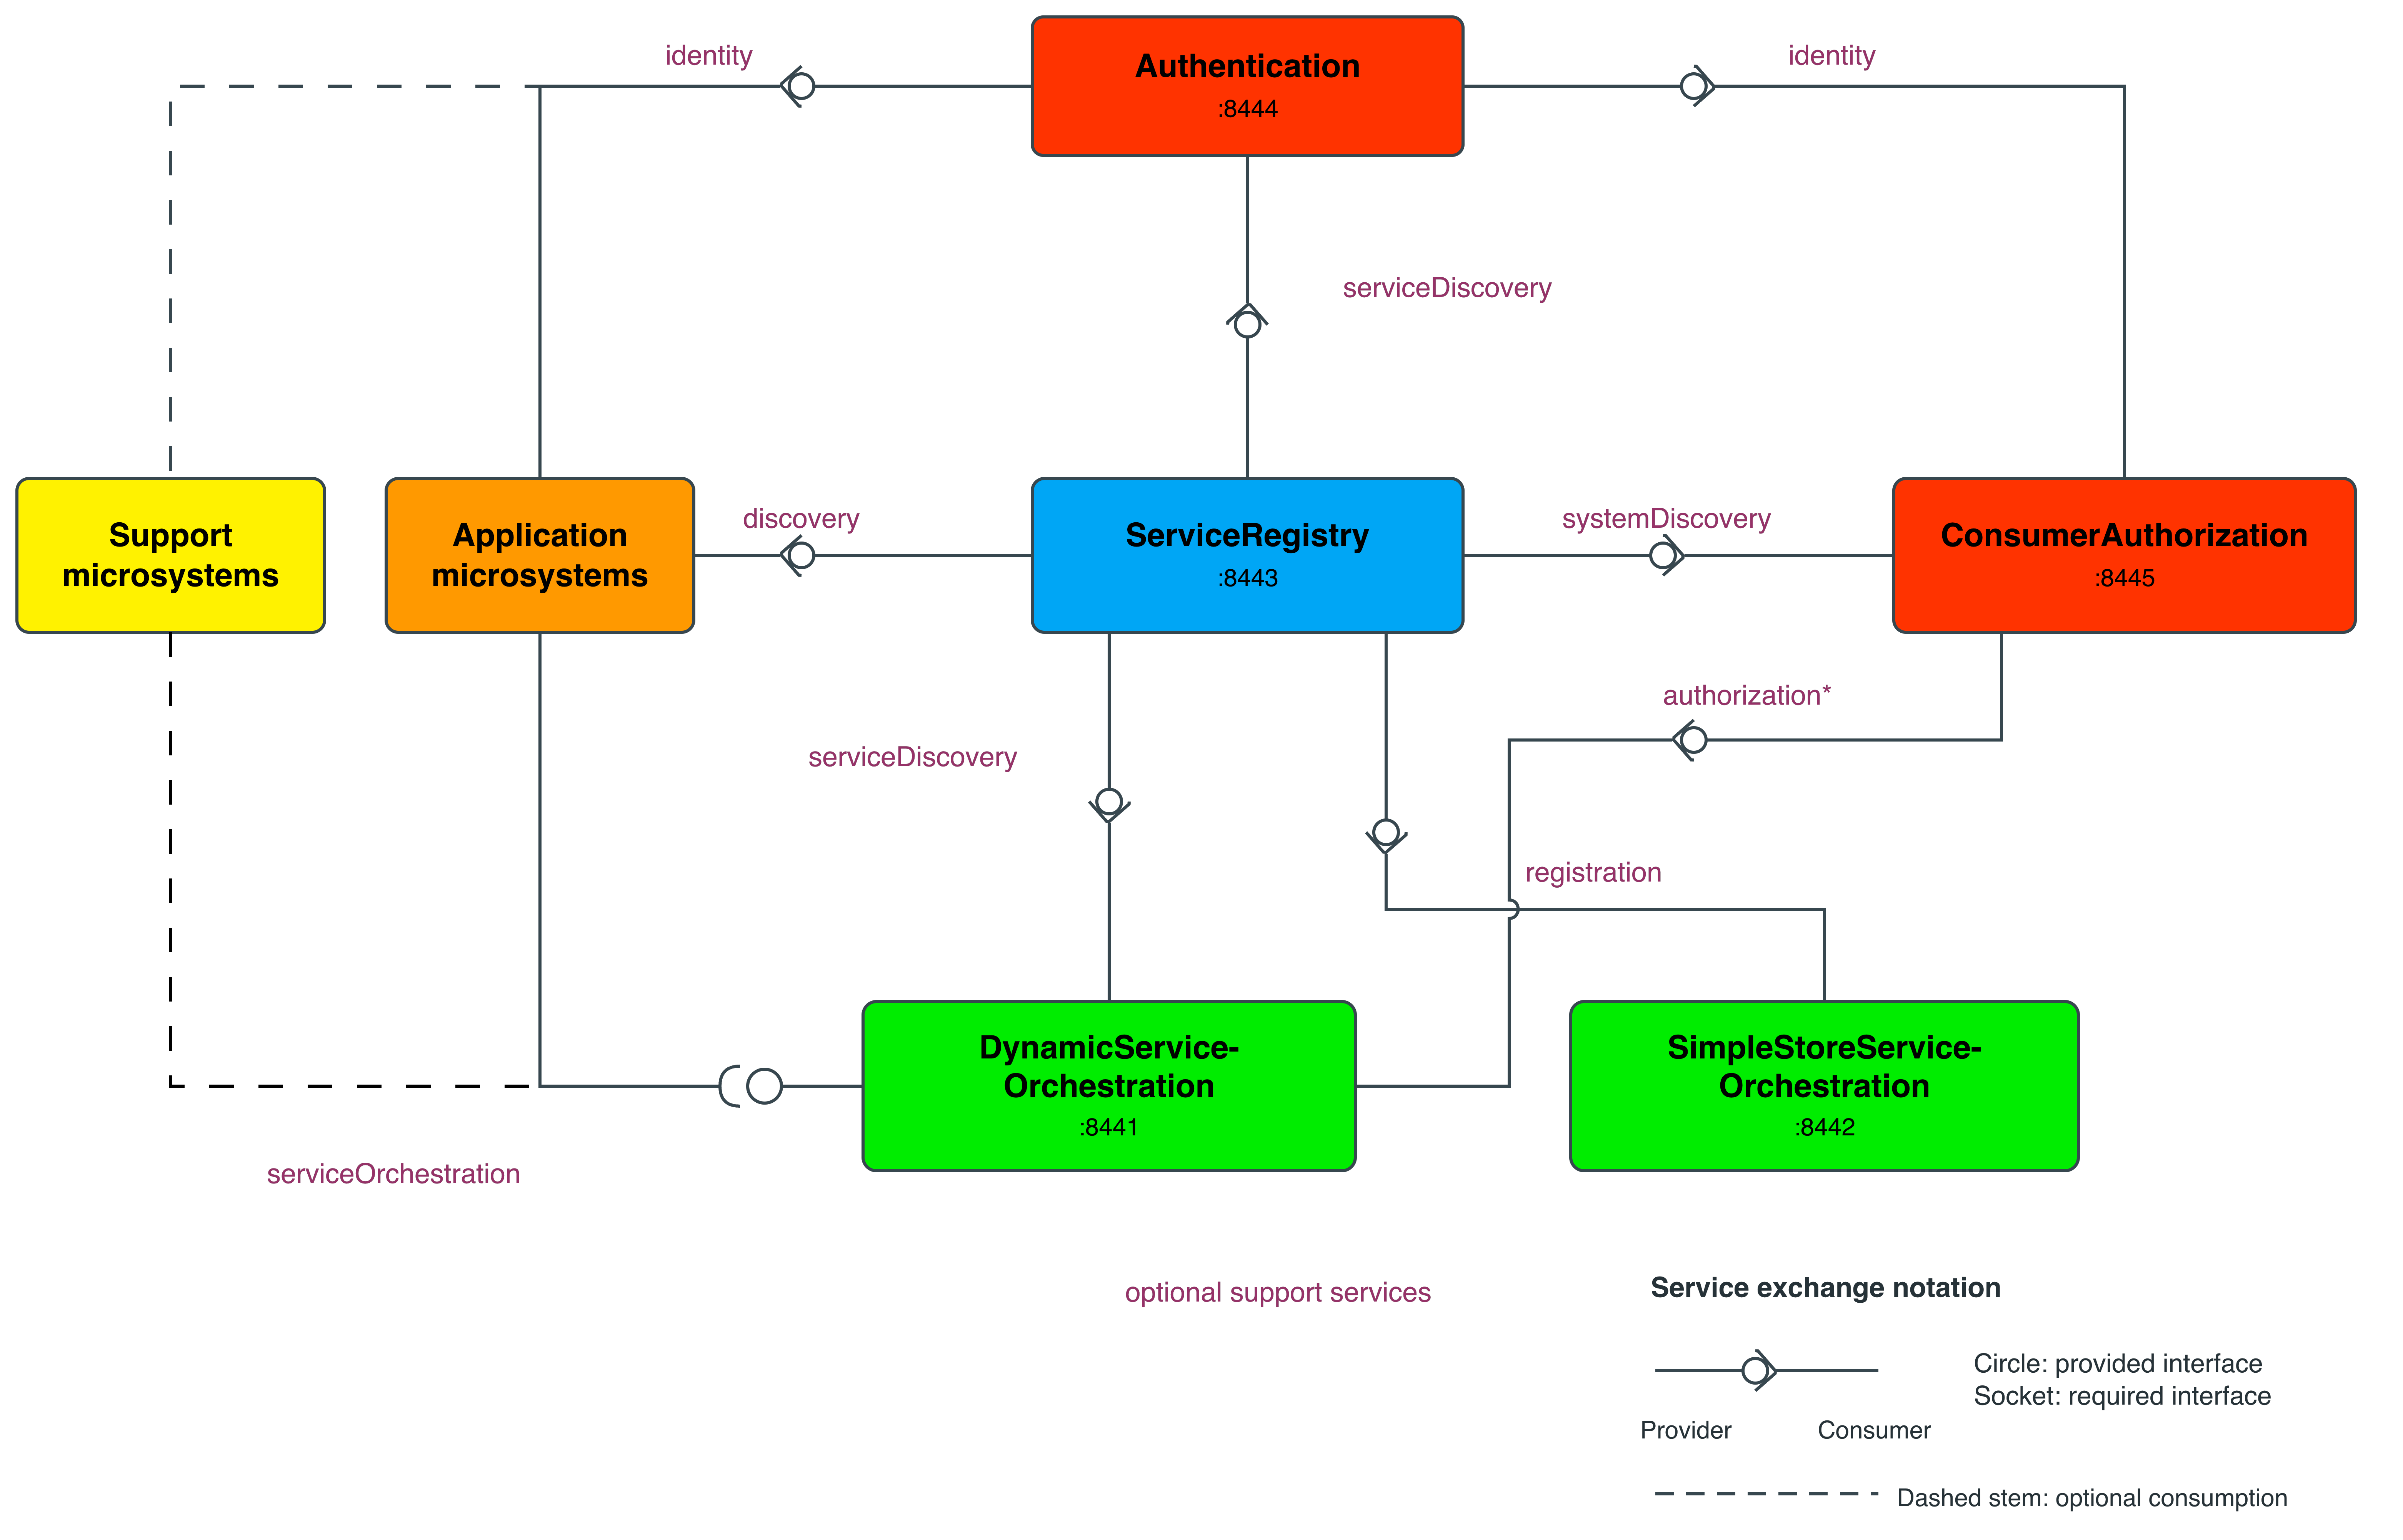
\includegraphics[width=\textwidth]{figures/figure-2-service-exchanges-v2.png}
 \begin{tikzpicture}[scale=0.9, every node/.style={transform shape}]
   \node[sysbox, ahRegistry] (sr)   at (0,0)     {ServiceRegistry\\[-2pt]{\scriptsize\normalfont :8443}};
   \node[sysbox, ahAuthentication] (auth) at (0,3.0)   {Authentication\\[-2pt]{\scriptsize\normalfont :8444}};
   \node[sysbox, ahAuthorization] (ca)   at (6.2,0)   {ConsumerAuthorization\\[-2pt]{\scriptsize\normalfont :8445}};
   \node[appbox, ahApplication] (app)  at (-6.2,0)  {Application\\microsystems};
   \node[sysbox, ahOrchestration] (dso)  at (-2.6,-3.0) {DynamicService-\\Orchestration\\[-2pt]{\scriptsize\normalfont :8441}};
   \node[sysbox, ahOrchestration] (sso)  at (3.4,-3.0)  {SimpleStoreService-\\Orchestration\\[-2pt]{\scriptsize\normalfont :8442}};
   \node[supbox] (bl)   at (-6.4,-6.0) {Blacklist\\[-2pt]{\scriptsize :8464}};
   \node[supbox, ahSupport] (tm)   at (-2.6,-6.0) {TranslationManager\\[-2pt]{\scriptsize :8465}};
   \node[supbox, ahSupport] (qos)  at (1.2,-6.0)  {DeviceQoSEvaluator\\[-2pt]{\scriptsize :8472}};

   \draw[uses] (auth) -- node[lbl, right]{\svc{serviceDiscovery}} (sr);
   \draw[uses] (ca) -- node[lbl, above]{\svc{systemDiscovery}} (sr);
   \draw[uses] (app) -- node[lbl, above]{discovery} (sr);
   \draw[uses] (dso) -- node[lbl, left, pos=0.45]{\svc{serviceDiscovery}} (sr);
   \draw[uses] (sso) -- node[lbl, right, pos=0.45]{registration} (sr);
   \draw[uses] (dso.north east) -- node[lbl, below right, pos=0.55]{\svc{authorization*}} (ca.south west);
   \draw[uses] (ca.north) |- node[lbl, above, pos=0.75]{\svc{identity}} (auth.east);
   \draw[uses] (app.north) |- node[lbl, above, pos=0.75]{\svc{identity}} (auth.west);
   \draw[uses] (app.south) |- node[lbl, below, pos=0.75]{\svc{serviceOrchestration}} (dso.west);
   \draw[opt] (dso.south west) -- (bl.north);
   \draw[opt] (dso) -- (tm);
   \draw[opt] (dso.south east) -- (qos.north);
 \end{tikzpicture}
 \caption{Component view of a 5.3.0 local cloud. Ports are the canonical ports of Section~\ref{sec:ports}.
 \svc{authorization*} denotes the \svc{authorizationManagement} and
 \svc{authorizationTokenManagement} services. Every Core system additionally consumes
 \svc{identity} when running with the \texttt{OUTSOURCED} authentication policy and
 \svc{authorization} when its management policy is \texttt{AUTHORIZATION}.}
 \label{fig:component}
\end{figure}

Typical deployments are:
 \begin{description}
   \item[Minimal (discovery only).] \sys{ServiceRegistry} alone; consumers look up providers
         directly (requires \prop{service.discovery.policy=open} or listing consumers in
         \prop{service.discovery.direct.access}).
   \item[Atomic orchestration.] \sys{ServiceRegistry} + \sys{SimpleStoreServiceOrchestration};
         operator-maintained, prioritised consumer$\rightarrow$instance rules. Consumers need
         discovery access to resolve the results (Section~\ref{sec:sso}).
   \item[Advanced orchestration.] \sys{ServiceRegistry} + \sys{DynamicServiceOrchestration}
         + \sys{ConsumerAuthorization} (+ \sys{Authentication}); orchestration returns complete
         access information including authorisation tokens.
   \item[Extended.] Advanced orchestration plus \sys{Blacklist}, \sys{TranslationManager}
         and/or \sys{DeviceQoSEvaluator}, enabled per feature flag.
 \end{description}


\subsection{Important Delimitations}
\label{sec:delimitations}

\begin{itemize}
  \item The document describes the \emph{tagged v5.3.0 release candidate}. 
  \item Only the five released Core microsystems are described in detail.
  \item \textcolor{red}{Only \emph{system} authentication is supported; user authentication is still under
        investigation (as stated in \cite{gsosd50}). The only \sys{Authentication} method is
        \prop{PASSWORD}.}
  \item \textcolor{red}{Onboarding and certificate issuing are outside the Core. Without them certificates must
        be provisioned out of band; with the \sys{Onboarding} and \sys{CertificateAuthority} Support
        systems they are issued through an operator-controlled onboarding procedure
        \cite{gsosddsup}.}
\end{itemize}

  
\section{SoS Functionalities and Properties}
\label{sec:properties}

\subsection{Functional properties of the SoS}
\begin{itemize}
  \item \textbf{Registry of devices, systems and service instances} with metadata, addresses,
        versions and typed interfaces (interface templates such as \prop{generic_http},
        \prop{generic_https}, \prop{generic_mqtt}, \prop{generic_mqtts}).
  \item \textbf{System identity} through X.509 certificates, self-declaration, or
        password login to \sys{Authentication} which issues
        time-limited identity tokens. Other authentication mechanisms .
  \item \textbf{Two-level access control} (management level overriding provider level) with
        policy types \prop{ALL}, \prop{WHITELIST}, \prop{BLACKLIST} and
        \prop{SYS_METADATA}, per service definition or event type and optionally per operation.
  \item \textbf{Access tokens}: time-limited, usage-limited and self-contained tokens
        (Base64 or RSA-SHA256/512 JSON Web Tokens), plus translation-bridge tokens.
  \item \textbf{Orchestration} in pull and push (subscription) mode, either rule-based from a
        prioritised store (atomic) or dynamically computed (advanced) with exclusivity
        locking, preferred providers, matchmaking, authorisation filtering, token issuing,
        and optional blacklist, QoS, translation and inter-cloud handling.
  \item \textbf{Uniform management}: every system exposes \svc{generalManagement}
        (\op{get-log}, \op{get-config}) and protects all \prop{/mgmt/} endpoints with a
        configurable management policy. Management here targets
        possible SW configuration and should be distinguish from
        monitoring (state, functionality, health, ...) 
\end{itemize}

\subsection{Configuration of SoS properties}
Each microsystem is configured by its own
\prop{application.properties} directed by the implementation language
used.

\subsubsection{Java configuration}
The key SoS-level properties based on the reference Java
implementation is summarized in Table~\ref{tab:config}. It's though
clear that these properties and effects need ot be addressed regardless of
implementation software language.

\begin{table}[h!]
\centering\footnotesize
\begin{tabularx}{\textwidth}{|P{4.6cm}|P{2.6cm}|Y|}\hline
\rowcolor{gray!33}Property & Secure default profile & Effect \\\hline
\prop{authentication.policy} & \prop{OUTSOURCED} with mTLS; \prop{CERTIFICATE} for an explicitly certificate-based binding & How a requester's identity is established: \prop{DECLARED}, \prop{CERTIFICATE}, \prop{OUTSOURCED}; \sys{Authentication} itself always uses \prop{INTERNAL}. \\\hline
\prop{server.ssl.enabled} & \prop{true}; client authentication required & Selects HTTPS/MQTTS and the \prop{generic_https}/\prop{generic_mqtts} interface templates. \\\hline
\prop{enable.management.filter}, \prop{management.policy}, \prop{management.whitelist} & \prop{true}, \prop{authorization} & Protection of \prop{/mgmt/} endpoints: \prop{SYSOP_ONLY}, \prop{WHITELIST}, \prop{AUTHORIZATION}. \\\hline
\prop{enable.blacklist.filter}, \prop{force.blacklist.filter} & \prop{false}, \prop{true} & Inbound requester check and orchestration candidate filtering against \sys{Blacklist}. \\\hline
\prop{service.discovery.policy}, \prop{service.discovery.direct.access} & \prop{restricted}; \prop{DynamicServiceOrchestration, TranslationManager, DeviceQoSEvaluator} & Whether arbitrary systems may look up arbitrary services in the \sys{ServiceRegistry}, or only those flagged \prop{unrestrictedDiscovery}. \\\hline
\prop{service.discovery.interface.policy} & \prop{restricted} & Handling of unknown interface templates on registration: \prop{restricted}, \prop{extendable}, \prop{open}. \\\hline
\prop{enable.authorization}, \prop{enable.translation}, \prop{enable.qos}, \prop{enable.intercloud} & \prop{true}, \prop{false}, \prop{false}, \prop{false} & Feature set of \sys{DynamicServiceOrchestration}. \\\hline
\prop{mqtt.api.enabled} & \prop{false} & Adds MQTT interfaces to all registered services. \\\hline
\prop{normalization.mode} & \prop{extended} & Automatic transformation of identifiers to the naming convention. \\\hline
\end{tabularx}
\caption{SoS-level switches for the default secure cloud profile. Component sample
values are not a statement of the architectural default; disabled security settings
are development exceptions. Other feature choices remain deployment-specific.}
\label{tab:config}
\end{table}

\subsubsection{GOlang configuration}


\subsubsection{Rust configuration}



\subsection{Data stored by the individual microsystems}
In line with the 5.x principle of relative system independence, every Core microsystem owns
a private database. Such databases should, long term, be capable
of storing semantic (RDF) triplet enabling semantically annotated
information interoperability.

\begin{table}[h!]
\centering\footnotesize
\begin{tabularx}{\textwidth}{|P{4.0cm}|P{3.6cm}|Y|}\hline
\rowcolor{gray!33}Microsystem & Schema & Persistent entities \\\hline
\sys{ServiceRegistry} & \prop{ah_serviceregistry} & Device, DeviceAddress, System, SystemAddress, DeviceSystemConnector, ServiceDefinition, ServiceInstance, ServiceInstanceInterface, ServiceInterfaceTemplate, ServiceInterfaceTemplateProperty, Logs \\\hline
\sys{Authentication} & \prop{ah_authentication} & System, PasswordAuthentication, ActiveSession, Logs \\\hline
\sys{ConsumerAuthorization} & \prop{ah_consumer_authorization} & AuthMgmtPolicyHeader, AuthProviderPolicyHeader, AuthPolicy, TokenHeader, TimeLimitedToken, UsageLimitedToken, SelfContainedToken, EncryptionKey, CryptographerAuxiliary, Logs \\\hline
\sys{DynamicServiceOrchestration} & \prop{ah_serviceorchestration_dynamic} & OrchestrationJob, OrchestrationLock, Subscription, QosEvalResult, OrchestrationPlantRules (local extension), Logs \\\hline
\sys{SimpleStoreServiceOrchestration} & \prop{ah_serviceorchestration_simple} & OrchestrationStore, OrchestrationJob, Subscription, Logs \\\hline
\end{tabularx}
\caption{Data ownership per Core microsystem.}
\label{tab:data}
\end{table}

\subsection{Non-functional properties}
\begin{itemize}
  \item \textbf{Security:} full AAA and encrypted communication are the default from
        v5.3; the reference profile uses mutual TLS, certificate-bound identity tokens,
        provider/operation authorisation and protected management. Implementation test
        modes are not equivalent default profiles. Token secrets and provider keys are
        additionally encrypted at rest in \sys{ConsumerAuthorization}.
        See Section~\ref{sec:security}.
  \item \textbf{Latency:} every request passes a filter chain which may call other systems
        (\svc{identity} \op{identity-verify} for outsourced authentication, \svc{authorization}
        \op{verify} for management requests, \svc{blacklistDiscovery}
        \op{check}). Policy  developers and management 
        should account for imposed extra round trips on the control plane.
  \textcolor{red}{\item \textbf{Scalability:} push orchestration is processed asynchronously by a bounded
        worker pool (\prop{push.orchestration.max.thread}); queries are paginated
        (\prop{max.page.size}, default 1000).}
  \item \textbf{Resource footprint:}  Available resources limits
    achievable properties like, e.g. compute performance, energy
    consumption, thus e.g. implementation languages will be a way of
    meeting use cae requirements.        
  \item \textbf{Safety and energy:} no specific mechanisms are
    speciifed and required yet.
\end{itemize}

\subsection{Stateful or stateless}
All Core microsystems are \emph{stateful} with respect to their persistent stores
(Table~\ref{tab:data}). Request handling itself is stateless except for: identity sessions
(\sys{Authentication}, expiring after \prop{identity.token.duration}, default 300\,s),
orchestration locks and push subscriptions (orchestration systems), and usage counters of
usage-limited tokens. Scheduled Quartz \emph{cleaner jobs} remove expired sessions, tokens,
locks, subscriptions and aged orchestration history.

\subsubsection{Access to microsystem state and logs}
Logs of individual microsystems can be retrieved through the
generalManagement service produced by all core systems. Microsystem
state can be addressed through the sysMonitor service produced by all
core systems. The state information varies between microsystem. A
harmonisation of state reporting is part of the roadmap work within
the Eclipse Arrowhead community.  

\textcolor{red}{REVIEWED TO HERE}


\newpage
%% ============================================================================================
\section{SoS Architecture}
\label{sec:architecture}

\subsection{Constituent Microsystems}

Table~\ref{tab:systems} maps the abstract Core systems of \cite{gsosd50} to the 5.3.0
microsystems.

\begin{table}[h!]
\centering\footnotesize
\begin{tabularx}{\textwidth}{|P{2.6cm}|P{4.6cm}|P{3.6cm}|P{0.8cm}|Y|}\hline
\rowcolor{gray!33}GSoSD 5.0 role & 5.3.0 microsystem & Module & Port & Approach \\\hline
Service Registry & \sys{ServiceRegistry} & \prop{serviceregistry} & 8443 & Bootstrap anchor; must start first \\\hline
Authentication system & \sys{Authentication} & \prop{authentication} & 8444 & Password login, identity tokens \\\hline
Authorisation system & \sys{ConsumerAuthorization} & \prop{consumer-authorization} & 8445 & Policy engine and token engine \\\hline
Orchestration system (advanced) & \sys{DynamicServiceOrchestration} & \prop{serviceorchestration-dynamic} & 8441 & Computed at request time \\\hline
Orchestration system (atomic) & \sys{SimpleStoreServiceOrchestration} & \prop{serviceorchestration-simple} & 8442 & Prioritised rule store \\\hline
\end{tabularx}
\caption{Mapping of abstract Core roles to 5.3.0 microsystems.}
\label{tab:systems}
\end{table}

As recommended by \cite{gsosd50}, a local cloud should run \emph{one} orchestration system.
Both orchestration systems produce the same \svc{serviceOrchestration} service definition
(same operations \op{pull}, \op{subscribe}, \op{unsubscribe}) and advertise their strategy
in the service metadata key \prop{orchestrationStrategy}, so consumers are independent
of the chosen approach.

\subsection{Common Internal Architecture of a Core Microsystem}
\label{sec:internal}

All Core microsystems share the same layered design as provided by
(Figure~\ref{fig:layers}).

\begin{figure}[h!]
\centering
\begin{tikzpicture}[node distance=0.12cm]
  \node[layer, fill=AHSysMLInterface, ahMixed] (api) {\textbf{API layer} -- HTTP REST controllers (\prop{api/http}) and MQTT topic handlers (\prop{api/mqtt})};
  \node[layer, fill=white, below=of api, ahMixed] (flt) {\textbf{Filter chain} -- authentication (15) $\rightarrow$ blacklist (20) $\rightarrow$ management (25)};
  \node[layer, below=of flt, ahMixed] (val) {\textbf{Validation \& normalisation} -- naming convention, DTO validation};
  \node[layer, below=of val, ahMixed] (svc) {\textbf{Service layer} -- business logic per produced service};
  \node[layer, below=of svc, ahMixed] (eng) {\textbf{Engines / drivers} -- policy engine, token engine, matchmaker, QoS driver, \ldots};
  \node[layer, below=of eng, ahMixed] (jpa) {\textbf{Persistence} -- JPA entities, repositories, DB services $\rightarrow$ private MySQL schema};
  \node[draw=ArrowheadGrey, fill=gray!6, minimum height=4.9cm, minimum width=3.3cm, align=center,
        font=\scriptsize, anchor=west] (cross) at ($(svc.east)+(0.3cm,0)$)
        {\textbf{Cross-cutting}\\[3pt]\prop{SystemInfo}\\(name, services,\\ policies)\\[3pt]
         \prop{ApplicationInitListener}\\(start-up, SR registration)\\[3pt]
         \prop{ServiceCollector}\\(cached service lookup)\\[3pt]
         \prop{ArrowheadHttpService}\\(outbound calls)\\[3pt]
         Quartz cleaner jobs};
\end{tikzpicture}
\caption{Internal layering shared by all 5.2.2 Core microsystems.}
\label{fig:layers}
\end{figure}

\begin{description}
  \item[SystemInfo.] Each microsystem has one \prop{SystemInfo} bean that defines its system
        name, its system model (address, version, metadata, X.509 public key when certificate
        authenticated) and the list of \prop{ServiceModel}s it produces. Interface models are
        generated from the actual configuration: HTTP or HTTPS template, domain name, port,
        base path and per-operation HTTP method and path; MQTT interfaces with base topics are
        added when \prop{mqtt.api.enabled=true}.
  \item[ApplicationInitListener.] At start-up the listener validates the server configuration,
        loads the key store and checks the server certificate against the Arrowhead
        certificate profile (secure mode), subscribes to MQTT topics, and -- for all systems except
        \sys{ServiceRegistry} -- checks the \sys{ServiceRegistry} connection (3 retries,
        15\,s apart), revokes any stale registration, registers the system and then each of
        its services. On shutdown it revokes its services and, if outsourced, logs out.
  \item[ServiceCollector.] Outbound consumption is name-based: a caller asks for
        \emph{service definition + operation}; the collector resolves the provider via the
        \sys{ServiceRegistry} (mode \prop{SR_ONLY}) or via \sys{ServiceRegistry} and
        orchestration (\prop{SR_AND_ORCH}, default) and caches the resolved model.
  \item[Cleaner jobs.] Quartz jobs periodically purge expired data (sessions, tokens,
        locks, subscriptions, history).
\end{description}

\subsection{Request Filter Chain}
\label{sec:filterchain}

Every inbound HTTP request (and, equivalently, every MQTT message) passes the ordered filter
chain of Figure~\ref{fig:filters} before reaching a controller. The authentication filter
sets two request attributes -- the \emph{authenticated system name} and the \emph{sysop}
flag -- on which all later decisions are based.

\begin{figure}[h!]
\centering
\begin{tikzpicture}[node distance=0.85cm]
  \node[appbox, minimum width=1.8cm, ahMixed] (req) {Request};
  \node[flt, right=of req, ahAuthentication] (a) {\textbf{Authentication}\\(order 15)\\Certificate / Outsourced\\TLS-protected};
  \node[flt, right=of a] (b) {\textbf{Blacklist}\\(order 20)\\if enabled};
  \node[flt, right=of b] (c) {\textbf{Management}\\(order 25)\\only \prop{/mgmt/} paths};
  \node[sysbox, minimum width=1.8cm, right=of c, ahMixed] (ctl) {API};
  \draw[msg] (req) -- (a); \draw[msg] (a) -- (b); \draw[msg] (b) -- (c); \draw[msg] (c) -- (ctl);
  \node[font=\scriptsize, below=0.15cm of a, text width=2.7cm, align=center] {401 if identity missing/invalid; 403 if foreign cloud or wrong cert type};
  \node[font=\scriptsize, below=0.15cm of b, text width=2.7cm, align=center] {\svc{blacklistDiscovery} \op{check}; 403 if listed (or if unreachable and forced)};
  \node[font=\scriptsize, below=0.15cm of c, text width=2.7cm, align=center] {sysop / whitelist / \svc{authorization} \op{verify}; 403 otherwise};
\end{tikzpicture}
\caption{Ordered inbound filter chain (\texttt{arrowhead-common}), reached after
TLS peer authentication and decryption. Provider/service authorisation remains
required after identity verification; it is not replaced by the management filter.}
\label{fig:filters}
\end{figure}

\paragraph{Authentication filters.}
\begin{itemize}
  \item \textbf{SelfDeclaredFilter (\prop{DECLARED})}: expects
        \prop{Authorization: Bearer SYSTEM//<SystemName>}. The name is trusted as given; the
        name \prop{Sysop} yields operator rights. Intended for development only.
  \item \textbf{CertificateFilter (\prop{CERTIFICATE})}: requires mutual TLS. The client
        certificate must have the \prop{SYSTEM} (\prop{sy}) or \prop{OPERATOR}
        (\prop{op}) profile type and belong to the same local cloud as the server (compared
        on the common name). The system name is derived from the CN; an operator certificate
        yields sysop rights.
  \item \textbf{OutsourcedFilter (\prop{OUTSOURCED})}: accepts
        \prop{Bearer IDENTITY-TOKEN//<token>}, verified by calling
        \svc{identity}~\op{identity-verify} on \sys{Authentication}, or
        \prop{Bearer AUTHENTICATOR-KEY//<SystemName>//<HMAC>} for systems sharing a secret key
        (used by \sys{Authentication} itself). A \sys{ServiceRegistry} lookup of exactly the
        \svc{identity} service may proceed without an identity token to break the bootstrap
        cycle; mutual TLS and peer/certificate checks still apply. This is not anonymous
        or unencrypted access.
\end{itemize}

\paragraph{Management filter.}
Requests whose path contains \prop{/mgmt/} are allowed according to
\prop{management.policy}: \prop{SYSOP_ONLY} (operator only), \prop{WHITELIST}
(operator or listed system), or \prop{AUTHORIZATION} (operator, listed system, or a positive
\svc{authorization}~\op{verify} answer from \sys{ConsumerAuthorization} for the service
definition and operation that the path and method map to).

\subsection{Local Cloud Bootstrapping}
\label{sec:bootstrap}

The v5.0-and-later baseline is full authentication, authorisation and audit (AAA) with
encrypted of exchanged information. The reference implementation must establish
that state before making ordinary services available. ServiceRegistry remains the
discovery anchor; this does not make Authentication, ConsumerAuthorization or
transport protection optional bootstrap additions.

\begin{enumerate}
  \item \textbf{Provision the protected foundation.} Create the private database
        schemas/users and install per-system certificates/private keys, trust stores,
        revocation material and bootstrap identity credentials. Configure
        \prop{server.ssl.enabled=true} and mutual TLS
        (\prop{server.ssl.client-auth=need}); publish protected HTTPS/MQTTS service
        bindings. The ServiceRegistry bootstrap address is configured through
        \prop{service.registry.address}/\prop{port}. An address is not a trust anchor.
  \item \textbf{Start protected discovery.} ServiceRegistry registers its own services
        in its database and exposes only the scoped bootstrap operations needed by
        the other Core systems. If a configured filter adds a support dependency,
        such as Blacklist, that dependency is also a readiness prerequisite.
        No anonymous or plaintext registry interval is required.
  \item \textbf{Bring AAA to readiness.} Start Authentication and ConsumerAuthorization
        with the provisioned identities, operator credentials and scoped initial
        policies. In the reference \prop{OUTSOURCED} profile, a system uses
        \prop{authenticator.credentials} to obtain an identity token over mutual TLS;
        verification binds that token to its certificate identity. A narrowly scoped
        lookup of \svc{identity} may precede possession of the token, but still requires
        authenticated, encrypted transport. Initial operator/certificate access and
        explicit bootstrap grants resolve dependency cycles without disabling AA.
  \item \textbf{Start authorised service selection.} Protect the selected orchestrator
        and ensure discovery, Authentication and ConsumerAuthorization are ready.
        DSO uses \prop{enable.authorization=true}; provision SimpleStore rules where
        that strategy is used. Those rules do not themselves grant service access. DSO's
        own authorisation/blacklist bootstrap lookups are scoped exceptions to
        recursive orchestration, not exceptions to the security baseline.
  \item \textbf{Release Support and application traffic.} Systems register their
        protected service offers and consume only permitted operations. Providers
        enforce the verified identity and policy/token decision even after
        orchestration. Missing trust, an invalid credential or an unavailable required
        AA decision prevents readiness or denies the request; startup does not fall
        back to \prop{DECLARED}, plaintext transport or unauthorised
        service use.
   \item \textbf{Start Audit} to be further defined and part of a
     later release. The task has currently been deferred to the roadmap WorkingGroup. 
        
\end{enumerate}

This sequence describes security and dependency readiness, not a strict process
ordering for every runtime. Registration, identity and policy bootstrap can require
controlled retries under the same security constraints. Unencrypted HTTP/MQTT,
self-declared identities and authorisation bypass are explicit isolated-test
exceptions; they are not the v5.0 default and do not demonstrate a conforming
local-cloud startup.

\newpage
%% ============================================================================================



\section{Microsystem White-Box Descriptions}
\label{sec:systems}

\subsection{ServiceRegistry}
\label{sec:sr}

\paragraph{Purpose.} Holds the authoritative registry of \emph{devices}, \emph{systems},
\emph{service definitions}, \emph{service instances} and \emph{interface templates} of the
local cloud. Compared with the abstract description in \cite{gsosd50}, 5.2.2 adds devices and
systems as first-class registry objects, so that physical deployment can be expressed.

\paragraph{Information model.}
A \emph{device} (name, addresses of type \prop{MAC}, \prop{IPV4}, \prop{IPV6},
\prop{HOSTNAME}, metadata) hosts one or more \emph{systems} (name, addresses, version,
metadata). A system provides \emph{service instances}; an instance is identified by
\prop{<SystemName>|<serviceDefinition>|<version>}, has an expiry time, metadata and one or
more \emph{interfaces}. Each interface instantiates an \emph{interface template} whose
\emph{template properties} (with mandatory flags and optional validators) constrain the
interface properties, e.g.\ \prop{accessAddresses}, \prop{accessPort},
\prop{basePath}, \prop{operations} for \prop{generic_http(s)}. Each interface also
carries a \emph{policy} (\prop{NONE}, \prop{CERT_AUTH}, \prop{TIME_LIMITED_TOKEN_AUTH},
\prop{USAGE_LIMITED_TOKEN_AUTH}, \prop{BASE64_SELF_CONTAINED_TOKEN_AUTH},
\prop{RSA_SHA256/512_JSON_WEB_TOKEN_AUTH}, \prop{TRANSLATION_BRIDGE_TOKEN_AUTH})
which tells the orchestration which kind of token a consumer needs.

\paragraph{Produced services.}
\svc{deviceDiscovery}, \svc{systemDiscovery} and \svc{serviceDiscovery}
(each \op{register}, \op{lookup}, \op{revoke}; flagged \prop{unrestrictedDiscovery}),
\svc{serviceRegistryManagement} (bulk CRUD on devices, systems, service definitions, service
instances and interface templates) and \svc{generalManagement}.

\paragraph{Key behaviour.}
\begin{itemize}
  \item \textbf{Registration ownership}: a system may only register/revoke itself and its own
        service instances (the requester's authenticated name must match).
  \item \textbf{Discovery policy}: with \prop{restricted} (default), a \op{lookup} by an
        ordinary system returns only instances whose metadata carries
        \prop{unrestrictedDiscovery=true} (i.e.\ the public Core services). Systems in
        \prop{service.discovery.direct.access} (by default \sys{DynamicServiceOrchestration},
        \sys{TranslationManager}, \sys{DeviceQoSEvaluator}) may look up everything. This
        forces application consumers to use orchestration, which applies authorisation.
  \item \textbf{Interface policy}: \prop{restricted} rejects unknown interface templates;
        \prop{extendable} creates a template with all supplied properties mandatory;
        \prop{open} creates an unconstrained template.
  \item \textbf{Address policy}: \prop{allow.self.addressing} and
        \prop{allow.non.routable.addressing} decide whether loopback/link-local and private
        addresses are accepted.
  \item \textbf{Verbose lookup}: with \prop{discovery.verbose=true}, a lookup may embed
        provider system and device details in the response.
\end{itemize}

\subsection{Authentication}
\label{sec:authn}

\paragraph{Purpose.} Issues and validates system identities when certificates are not used
(\prop{OUTSOURCED} policy in the other systems). It realises the \emph{Authentication system}
of \cite{gsosd50} for dynamic, token-based identities.

\paragraph{Produced services.}
\svc{identity} (\op{identity-login}, \op{identity-logout}, \op{identity-change-credentials},
\op{identity-verify}; unrestricted discovery), \svc{identityManagement}
(\op{identity-mgmt-create}, \op{identity-mgmt-update}, \op{identity-mgmt-remove},
\op{identity-mgmt-query}, \op{identity-mgmt-session-close}, \op{identity-mgmt-session-query})
and \svc{generalManagement}.

\paragraph{Key behaviour.}
\begin{itemize}
  \item Identities (system name, sysop flag, authentication method \prop{PASSWORD} and
        hashed credentials) are created by the operator through \svc{identityManagement}.
  \item \op{identity-login} validates the credentials and opens an \emph{ActiveSession} with a
        random identity token valid for \prop{identity.token.duration} seconds (default 300).
        The client presents the token as \prop{Bearer IDENTITY-TOKEN//<token>}.
  \item \op{identity-verify} returns whether a token is valid and, if so, the system name and
        sysop flag -- used by the \prop{OutsourcedFilter} of every other system.
  \item \sys{Authentication} runs with the fixed \prop{INTERNAL} policy. Its own outbound
        calls use an \emph{authenticator key}, an HMAC of its system name with
        \prop{authentication.secret.key}, which the other systems hold in
        \prop{authenticator.secret.keys}.
  \item A cleaner job removes expired sessions every \prop{cleaner.job.interval} ms.
\end{itemize}

\subsection{ConsumerAuthorization}
\label{sec:authz}

\paragraph{Purpose.} Realises the \emph{Authorisation system}: stores access-control policies,
answers access checks and issues and verifies access tokens.

\paragraph{Produced services.}
\begin{itemize}
  \item \svc{authorization} (\op{grant}, \op{revoke}, \op{lookup}, \op{verify}; unrestricted):
        providers grant/revoke \emph{provider-level} policies for their own services; anyone
        may verify.
  \item \svc{authorizationToken} (\op{generate}, \op{verify}, \op{get-public-key},
        \op{register-encryption-key}, \op{unregister-encryption-key}; unrestricted).
  \item \svc{authorizationManagement} (\op{grant-policies}, \op{revoke-policies},
        \op{query-policies}, \op{check-policies}): \emph{management-level} policies.
  \item \svc{authorizationTokenManagement} (\op{generate-tokens}, \op{query-tokens},
        \op{revoke-tokens}, \op{add-encryption-keys}, \op{remove-encryption-keys}).
  \item \svc{generalManagement}.
\end{itemize}

\paragraph{Policy engine.} A policy header identifies
\emph{(cloud, provider, target type, target)}, where the target type is
\prop{SERVICE_DEF} or \prop{EVENT_TYPE}; it holds a default policy and optional
per-operation (scope) policies. A policy is \prop{ALL}, \prop{WHITELIST} (list of
consumers), \prop{BLACKLIST} (list of consumers) or \prop{SYS_METADATA} (a metadata
requirement evaluated against the consumer's metadata, fetched from the
\sys{ServiceRegistry} through \svc{systemDiscovery}~\op{lookup}). Evaluation
(Figure~\ref{fig:policy}) implements the GSoSD priority rule: management-level policies,
set by the operator, override provider-level policies set by the application provider; if
neither level has a relevant policy, access is denied.

\begin{figure}[h!]
\centering
\begin{tikzpicture}[node distance=0.35cm]
  \node[pstep, ahAuthorization] (s1) {1.\ Find relevant \textbf{MGMT-level} policies for (consumer, provider, target, operation)};
  \node[pstep, below=of s1, ahAuthorization] (s2) {2.\ Evaluate: all match $\Rightarrow$ \prop{TRUE}; any mismatch $\Rightarrow$ \prop{FALSE}; none $\Rightarrow$ \prop{UNDECIDED}};
  \node[pstep, below=of s2, ahAuthorization] (s3) {3.\ If \prop{UNDECIDED}: find relevant \textbf{PROVIDER-level} policies};
  \node[pstep, below=of s3, ahAuthorization] (s4) {4.\ Evaluate as in 2; \prop{UNDECIDED} $\Rightarrow$ \textbf{deny}};
  \draw[msg] (s1) -- (s2); \draw[msg] (s2) -- (s3); \draw[msg] (s3) -- (s4);
\end{tikzpicture}
\caption{Access decision in \texttt{AuthorizationPolicyEngine}.}
\label{fig:policy}
\end{figure}

\paragraph{Token engine.} Tokens are bound to (consumer, provider, target, scope):
\begin{itemize}
  \item \textbf{time-limited} (expires after \prop{token.time.limit}, default 60\,s) and
        \textbf{usage-limited} (\prop{simple.token.usage.limit} uses, default 5) simple tokens
        of \prop{simple.token.byte.size} bytes;
  \item \textbf{self-contained} tokens, Base64 or JWT signed with the system's RSA key
        (SHA-256/512), verifiable offline using \op{get-public-key};
  \item \textbf{translation-bridge} tokens, used only by \sys{TranslationManager}.
\end{itemize}
A provider can register an encryption key, after which tokens issued for its services are
returned encrypted for it. Token secrets and provider keys are stored encrypted with
\prop{secret.cryptographer.key}. Systems listed in
\prop{unbounded.token.generation.whitelist} (by default \sys{DynamicServiceOrchestration} and
\sys{TranslationManager}) may generate tokens on behalf of other consumers. Tokens are
deleted after \prop{token.max.age} minutes.

\subsection{DynamicServiceOrchestration}
\label{sec:dso}

\paragraph{Purpose.} Realises the \emph{advanced} orchestration approach of \cite{gsosd50}: it
computes at request time which provider instances a consumer should use and returns
everything needed to consume them (addresses, interfaces, tokens).

\paragraph{Produced services.}
\svc{serviceOrchestration} (\op{pull}, \op{subscribe}, \op{unsubscribe}; unrestricted
discovery), \svc{serviceOrchestrationPushManagement}
(\op{subscribe}, \op{unsubscribe}, \op{trigger}, \op{query}),
\svc{serviceOrchestrationLockManagement} (\op{create}, \op{query}, \op{remove}),
\svc{serviceOrchestrationHistoryManagement} (\op{query}) and \svc{generalManagement}.
The system and its \svc{serviceOrchestration} service carry the metadata key
\prop{orchestrationStrategy}.

\paragraph{Orchestration request.} An \emph{orchestration form} names the target service
definition and optionally operations, versions, interface templates and properties, security
policies, metadata requirements, preferred providers, QoS requirements, an exclusivity
duration and orchestration \emph{flags}: \prop{MATCHMAKING}, \prop{ONLY_PREFERRED},
\prop{ONLY_EXCLUSIVE}, \prop{ALLOW_TRANSLATION}, \prop{ALLOW_INTERCLOUD},
\prop{ONLY_INTERCLOUD}. Each pull or push creates an \emph{OrchestrationJob} record
(the orchestration history).

\paragraph{Local orchestration pipeline.} Figure~\ref{fig:dso} shows the candidate pipeline
implemented in \prop{LocalServiceOrchestration}. Each step can only remove candidates;
an empty set terminates the job with an empty result and warnings.

\begin{figure}[h!]
\centering
\begin{tikzpicture}[node distance=0.16cm]
  \node[pstep, ahOrchestration] (p1) {1.\ \textbf{Service discovery}: \svc{serviceDiscovery}~\op{lookup} on \sys{ServiceRegistry}};
  \node[pstep, below=of p1, ahOrchestration] (p2) {2.\ Remove instances \textbf{locked} by other consumers};
  \node[pstep, below=of p2, ahOrchestration] (p3) {3.\ \textbf{Exclusivity}: mark/keep instances with \prop{allowExclusivity}};
  \node[pstep, below=of p3, ahOrchestration] (p4) {4.\ \textbf{Blacklist} cross-check (\svc{blacklistManagement}~\op{query})};
  \node[pstep, below=of p4, ahOrchestration] (p5) {5.\ \textbf{Authorisation} cross-check (\svc{authorizationManagement}~\op{check-policies})};
  \node[pstep, below=of p5, ahOrchestration] (p6) {6.\ Temporary \textbf{lock} of exclusive candidates (60\,s)};
  \node[pstep, below=of p6, ahOrchestration] (p7) {7.\ Keep \textbf{interface-compatible} candidates};
  \node[pstep, below=of p7, ahOrchestration] (p8) {8.\ \textbf{Translation}: prefer native; else \svc{translationBridgeManagement}~\op{discovery}};
  \node[pstep, below=of p8, ahOrchestration] (p9) {9.\ \textbf{Preferences}: reservable, then preferred providers};
  \node[pstep, below=of p9, ahOrchestration] (p10) {10.\ \textbf{QoS} filter/sort (\svc{qualityEvaluation} on \sys{DeviceQoSEvaluator})};
  \node[pstep, below=of p10, ahOrchestration] (p11) {11.\ \textbf{Matchmaking}: choose one; release other temporary locks};
  \node[pstep, below=of p11, ahOrchestration] (p12) {12.\ \textbf{Tokens}: \svc{authorizationTokenManagement}~\op{generate-tokens}};
  \node[pstep, below=of p12, ahOrchestration] (p13) {13.\ \textbf{Bridge}: \svc{translationBridgeManagement}~\op{negotiation}};
  \foreach \a/\b in {p1/p2,p2/p3,p3/p4,p4/p5,p5/p6,p6/p7,p7/p8,p8/p9,p9/p10,p10/p11,p11/p12,p12/p13} \draw[msg] (\a) -- (\b);
  \node[cond, right=0.4cm of p4] {only if \prop{enable.blacklist.filter}};
  \node[cond, right=0.4cm of p5] {\prop{enable.authorization=true}\\default secure profile};
  \node[cond, right=0.4cm of p8] {only if \prop{enable.translation} and flag \prop{ALLOW_TRANSLATION}};
  \node[cond, right=0.4cm of p10] {only if QoS requirements given; requires \prop{enable.qos}};
  \node[cond, right=0.4cm of p11] {only if \prop{MATCHMAKING} (set implicitly by exclusivity/translation)};
  \node[cond, right=0.4cm of p12] {AA enabled; token path when no bridge};
\end{tikzpicture}
\caption{Candidate pipeline of \sys{DynamicServiceOrchestration} (local cloud).}
\label{fig:dso}
\end{figure}

\paragraph{Push orchestration.} Consumers (or operators, via push management) create
\emph{subscriptions} with a notify interface (\prop{HTTP}, \prop{HTTPS}, \prop{MQTT},
\prop{MQTTS}) and optional duration. A \op{trigger} (or an immediate trigger at
subscription time) queues jobs that a bounded worker pool executes, delivering results to
the subscriber. \textbf{Locks} reserve exclusive instances until their expiry and can be
managed by operators. A cleaner job removes expired subscriptions and locks and history
older than \prop{orchestration.history.max.age} days.

\subsection{SimpleStoreServiceOrchestration}
\label{sec:sso}

\paragraph{Purpose.} Realises the \emph{atomic} orchestration approach of \cite{gsosd50}:
an operator-maintained table maps consumers to concrete service instances.

\paragraph{Produced services.} \svc{serviceOrchestration} (\op{pull}, \op{subscribe},
\op{unsubscribe}), \svc{serviceOrchestrationSimpleStoreManagement} (\op{create},
\op{query}, \op{remove}, \op{modify-priorities}), \svc{serviceOrchestrationPushManagement},
\svc{serviceOrchestrationHistoryManagement} and \svc{generalManagement}.

\paragraph{Key behaviour.} Each \emph{OrchestrationStore} rule is
(consumer, service definition, service instance identifier, priority). A pull returns the
consumer's rules for the requested service definition ordered by priority, re-ordered by
preferred providers (\prop{ONLY_PREFERRED} drops others), and reduced to the
highest-priority rule per service definition with \prop{MATCHMAKING}. The response contains
only the instance identifier, provider name, service definition and version; the
consumer resolves access details itself (from the \sys{ServiceRegistry} or local configuration).
The system consumes no other Core services during orchestration; consequently it does not
check authorisation or issue tokens, and keeping rules consistent with the registry is the
operator's task -- exactly the trade-off identified in \cite{gsosd50}.

\paragraph{Restricted discovery.} A \op{lookup} of an instance identifier under the default
\prop{restricted} policy returns only instances marked \prop{unrestrictedDiscovery}. Other
instances are missing from the result, with no error. Three combinations are intended:
\begin{itemize}
  \item \sys{DynamicServiceOrchestration} for ordinary consumers. This is the recommended
        default, because results carry complete access information and no consumer needs
        discovery access.
  \item \prop{restricted} with each \sys{SimpleStoreServiceOrchestration} consumer listed in
        \prop{service.discovery.direct.access}. A listed consumer can discover every service,
        so providers must still check it.
  \item \prop{open}, only in an isolated cloud where every system may discover every service.
\end{itemize}
A consumer that holds the access details in local configuration needs no \op{lookup} and no
discovery access.

\subsection{Interacting Support Systems (5.3.0}
\label{sec:support}

\begin{table}[h!]
\centering\footnotesize
\begin{tabularx}{\textwidth}{|P{3.2cm}|P{0.8cm}|P{5.0cm}|Y|}\hline
\rowcolor{gray!33}Support system & Port & Produced services & Used by the Core \\\hline
\sys{Blacklist} & 8464 & \svc{blacklistDiscovery}, \svc{blacklistManagement}, \svc{generalManagement} & Blacklist filter of every Core system (\op{check}); \sys{DynamicServiceOrchestration} candidate filtering (\op{query}). \\\hline
\sys{TranslationManager} & 8465 & \svc{translationBridge}, \svc{translationBridgeManagement}, \svc{translationReport}, \svc{generalManagement} & \sys{DynamicServiceOrchestration} interface/data-model translation (\op{discovery}, \op{negotiation}). \\\hline
\sys{DeviceQoSEvaluator} & 8472 & \svc{qualityEvaluation}, \svc{deviceQualityDataManagement}, \svc{generalManagement} & \sys{DynamicServiceOrchestration} QoS filtering/sorting. \\\hline
\end{tabularx}
\caption{5.2.2 Support systems the Core interacts with.}
\label{tab:support}
\end{table}

\newpage
%% ============================================================================================

\subsection{Plant-Managed Dynamic Orchestration (Local Extension)}
\label{sec:pde-dso}
The PDE backend uses
\sys{DynamicServiceOrchestration}. PDE atomically publishes the complete active-plant
snapshot using \svc{serviceOrchestrationPlantManagement}: \op{query} is
\prop{POST /serviceorchestration/mgmt/plant-rules/query}; \op{replace} is
\prop{PUT /serviceorchestration/mgmt/plant-rules/replace}. This is a local Java extension;
it is not part of the unmodified upstream 5.3.0 contract.

A scope is a consumer and service definition with ranked service-instance identifiers.
Lower nonnegative priority wins among eligible providers. Empty provider lists retain managed
scopes with no result; an empty scope list clears the active plant. DSO first restricts
candidates to the engineered set, then retains its normal authorisation, blacklist, lock,
interface and QoS checks. With matchmaking, it selects the best surviving plant priority;
without matchmaking it returns the survivors in priority order. Consumer preferences can
narrow this set, but cannot introduce an unengineered provider. Managed scopes cannot escape
through local failure, \texttt{ALLOW\_INTERCLOUD} or \texttt{ONLY\_INTERCLOUD}.

The \prop{orchestration_plant_rules} table stores one atomic snapshot in DSO's database,
retaining it across restarts. Replacement requires both management-policy permission and
an authenticated PDE or Sysop identity; LocalCloudManager may query only. PDE retains its
own plant-description and alarm stores. An unresolved producer produces an empty managed
scope, rather than deleting the consumer's engineering constraint. No active description
clears the snapshot. Query/replacement failures leave PDE degraded rather than claiming
that the plant is in force.

Apply \prop{database_patch_pde_dso.sql} to an existing DSO database before starting the
upgraded runtime. The Java test-cloud migration target creates the table and grants data
access, and configures operation-scoped query/replace permissions. Verify PDE's successful
synchronisation before relying on the new constraints. Existing consumer orchestration
caches (normally 300\,s) can delay visible changes beyond the PDE's 15\,s interval.
Legacy PDE-owned SSO entries are not automatically deleted; optional cleanup must preserve
operator-owned SSO rules. SimpleStore remains an independent optional backend, but PDE no
longer requires it. This update records source/configuration changes, not a live deployment
or cross-language conformance result.

\section{Services}
\label{sec:services}

All services are versioned \prop{1.0.0} and are offered over \prop{generic_http} or
\prop{generic_https} (depending on \prop{server.ssl.enabled}) and, when enabled, over
\prop{generic_mqtt}/\prop{generic_mqtts}. The service-specific SD and IDD documents
are published in the implementation documentation \cite{ah5docs}.

\subsection{Produced Services}

{\footnotesize
\begin{longtable}{|P{3.0cm}|P{4.3cm}|P{4.6cm}|P{3.8cm}|}\hline
\rowcolor{gray!33}Microsystem & Service definition & Operations & HTTP base path \\\hline\endhead
\multirow{5}{*}{\sys{ServiceRegistry}}
 & \svc{deviceDiscovery}$^\dagger$ & register, lookup, revoke & \prop{/serviceregistry/device-discovery} \\\cline{2-4}
 & \svc{systemDiscovery}$^\dagger$ & register, lookup, revoke & \prop{/serviceregistry/system-discovery} \\\cline{2-4}
 & \svc{serviceDiscovery}$^\dagger$ & register, lookup, revoke & \prop{/serviceregistry/service-discovery} \\\cline{2-4}
 & \svc{serviceRegistryManagement} & device-, system-, service-definition-, service-, interface-template- query/create/(update)/remove & \prop{/serviceregistry/mgmt} \\\cline{2-4}
 & \svc{generalManagement} & get-log, get-config & \prop{/serviceregistry/general/mgmt} \\\hline
\multirow{3}{*}{\sys{Authentication}}
 & \svc{identity}$^\dagger$ & identity-login, identity-logout, identity-change-credentials, identity-verify & \prop{/authentication/identity} \\\cline{2-4}
 & \svc{identityManagement} & identity-mgmt-create/-update/-remove/-query, identity-mgmt-session-close/-query & \prop{/authentication/mgmt} \\\cline{2-4}
 & \svc{generalManagement} & get-log, get-config & \prop{/authentication/general/mgmt} \\\hline
\multirow{5}{3cm}{\raggedright\sys{ConsumerAuthorization}}
 & \svc{authorization}$^\dagger$ & grant, revoke, lookup, verify & \prop{/consumerauthorization/authorization} \\\cline{2-4}
 & \svc{authorizationToken}$^\dagger$ & generate, verify, get-public-key, register-encryption-key, unregister-encryption-key & \prop{/consumerauthorization/ authorization-token} \\\cline{2-4}
 & \svc{authorizationManagement} & grant-policies, revoke-policies, query-policies, check-policies & \prop{/consumerauthorization/ authorization/mgmt} \\\cline{2-4}
 & \svc{authorizationTokenManagement} & generate-tokens, query-tokens, revoke-tokens, add-encryption-keys, remove-encryption-keys & \ldots\prop{/authorization/mgmt/token} \\\cline{2-4}
 & \svc{generalManagement} & get-log, get-config & \prop{/consumerauthorization/ general/mgmt} \\\hline
\multirow{6}{*}{\parbox{3cm}{\sys{DynamicService-}\\\sys{Orchestration}}}
 & \svc{serviceOrchestration}$^\dagger$ & pull, subscribe, unsubscribe & \prop{/serviceorchestration/ orchestration} \\\cline{2-4}
 & \svc{serviceOrchestrationPush\-Management} & subscribe, unsubscribe, trigger, query & \texttt{\ldots/mgmt/push} \\\cline{2-4}
 & \svc{serviceOrchestrationLock\-Management} & create, query, remove & \texttt{\ldots/mgmt/lock} \\\cline{2-4}
 & \svc{serviceOrchestrationHistory\-Management} & query & \texttt{\ldots/mgmt/history} \\\cline{2-4}
 & \svc{generalManagement} & get-log, get-config & \prop{/serviceorchestration/ general/mgmt} \\\hline
 & \svc{serviceOrchestrationPlantManagement} & query, replace & \prop{/serviceorchestration/mgmt/plant-rules} \\ \hline
\multirow{5}{*}{\parbox{3cm}{\sys{SimpleStoreService-}\\\sys{Orchestration}}}
 & \svc{serviceOrchestration}$^\dagger$ & pull, subscribe, unsubscribe & \prop{/serviceorchestration/ orchestration} \\\cline{2-4}
 & \svc{serviceOrchestrationSimple\-StoreManagement} & create, query, remove, modify-priorities & \texttt{\ldots/mgmt/simple-store} \\\cline{2-4}
 & \svc{serviceOrchestrationPush\-Management} & subscribe, unsubscribe, trigger, query & \texttt{\ldots/mgmt/push} \\\cline{2-4}
 & \svc{serviceOrchestrationHistory\-Management} & query & \texttt{\ldots/mgmt/history} \\\cline{2-4}
 & \svc{generalManagement} & get-log, get-config & \prop{/serviceorchestration/ general/mgmt} \\\hline
\caption{Services produced by the 5.2.2 Core microsystems. $^\dagger$ = registered with
\texttt{unrestrictedDiscovery=true} (directly discoverable in \texttt{restricted} mode).}
\label{tab:produced}
\end{longtable}
}

\subsection{Consumed Services}

{\footnotesize
\begin{longtable}{|P{3.6cm}|P{5.0cm}|P{6.9cm}|}\hline
\rowcolor{gray!33}Consumer & Service \& operation (provider) & When \\\hline\endhead
All except \sys{ServiceRegistry} & \svc{systemDiscovery}, \svc{serviceDiscovery}: register, revoke (\sys{ServiceRegistry}) & Start-up and shutdown (\prop{ApplicationInitListener}). \\\hline
All with \prop{OUTSOURCED} policy & \svc{identity}: identity-login, identity-logout (\sys{Authentication}) & Start-up/shutdown, to obtain own identity token. \\\hline
All with \prop{OUTSOURCED} policy & \svc{identity}: identity-verify (\sys{Authentication}) & Each inbound request (OutsourcedFilter). \\\hline
All with \prop{AUTHORIZATION} management policy & \svc{authorization}: verify (\sys{ConsumerAuthorization}) & Each inbound \prop{/mgmt/} request from a non-sysop, non-whitelisted system. \\\hline
All with blacklist filter & \svc{blacklistDiscovery}: check (\sys{Blacklist}) & Each inbound request. \\\hline
\sys{ConsumerAuthorization} & \svc{systemDiscovery}: lookup (\sys{ServiceRegistry}) & Evaluating \prop{SYS_METADATA} policies. \\\hline
\sys{DynamicServiceOrchestration} & \svc{serviceDiscovery}: lookup (\sys{ServiceRegistry}) & Every orchestration (step 1). \\\hline
\sys{DynamicServiceOrchestration} & \svc{authorizationManagement}: check-policies; \svc{authorizationTokenManagement}: generate-tokens (\sys{ConsumerAuthorization}) & When \prop{enable.authorization=true}. \\\hline
\sys{DynamicServiceOrchestration} & \svc{blacklistManagement}: query (\sys{Blacklist}) & When the blacklist filter is enabled. \\\hline
\sys{DynamicServiceOrchestration} & \svc{translationBridgeManagement}: discovery, negotiation (\sys{TranslationManager}) & When translation is enabled and allowed. \\\hline
\sys{DynamicServiceOrchestration} & \svc{qualityEvaluation} (\sys{DeviceQoSEvaluator}) & When QoS requirements are given and \prop{enable.qos=true}. \\\hline
\sys{SimpleStoreServiceOrchestration} & -- & No Core services consumed during orchestration. \\\hline
\caption{Services consumed by the 5.2.2 Core microsystems.}
\label{tab:consumed}
\end{longtable}
}

\newpage
%% ============================================================================================
\section{Use Cases (White Box)}
\label{sec:usecases}

The use cases of \cite{gsosd50} are revisited here with the concrete 5.2.2 services, operations
and filters. Numbered circles refer to the explanation below each diagram.

\subsection{Bootstrapping and Service Registration}

\begin{figure}[h!]
\centering
\begin{tikzpicture}[yscale=0.62]
  \seqhead{9.0}{0}{Provider A}{ahead, ahApplication}
  \seqhead{9.0}{5}{ServiceRegistry}{head, ahRegistry}
  \seqhead{9.0}{10}{Authentication}{head, ahAuthentication}
  \draw[msg] (0,-1.4) -- node[lbl, above]{\svc{serviceDiscovery}~\op{lookup}(identity)} (5,-1.4);
  \node[num] at (-0.4,-1.4) {1};
  \draw[ret] (5,-2.2) -- (0,-2.2);
  \draw[msg] (0,-3.2) -- node[lbl, above, pos=0.3]{\svc{identity}~\op{identity-login}(name, password)} (10,-3.2);
  \node[num] at (-0.4,-3.2) {2};
  \draw[ret] (10,-4.0) -- node[lbl, below, pos=0.3]{identity token} (0,-4.0);
  \draw[msg] (0,-5.2) -- node[lbl, above]{\svc{systemDiscovery}~\op{register} (Bearer IDENTITY-TOKEN)} (5,-5.2);
  \node[num] at (-0.4,-5.2) {3};
  \draw[msg] (5,-5.9) -- node[lbl, above]{\svc{identity}~\op{identity-verify}} (10,-5.9);
  \draw[ret] (10,-6.5) -- (5,-6.5);
  \draw[ret] (5,-7.0) -- (0,-7.0);
  \draw[msg] (0,-8.0) -- node[lbl, above]{\svc{serviceDiscovery}~\op{register}(a)} (5,-8.0);
  \node[num] at (-0.4,-8.0) {4};
  \draw[ret] (5,-8.7) -- (0,-8.7);
\end{tikzpicture}
\caption{Registration with certificate-bound \texttt{OUTSOURCED} authentication
on mutually authenticated, encrypted channels. TLS handshakes are omitted.}
\label{fig:uc-boot}
\end{figure}

\begin{enumerate}[leftmargin=*]
  \item[\textcircled{\scriptsize 1}] A looks up \svc{identity}; this exact bootstrap lookup does not require an identity
        token yet. It still requires mutual TLS and a trusted caller certificate.
  \item[\textcircled{\scriptsize 2}] A logs in and receives an identity token (default 300\,s).
  \item[\textcircled{\scriptsize 3}] A registers itself; the \sys{ServiceRegistry} verifies the
        token with \sys{Authentication} before accepting.
  \item[\textcircled{\scriptsize 4}] A registers its service \svc{a} with its interfaces and
        interface policy. With \prop{CERTIFICATE} policy steps 1--2 and the verification
        are replaced by certificate-derived identity on mutual TLS. The isolated
        \prop{DECLARED} test mode does not satisfy this secure use case. Provider/service
        authorisation remains required independently of the chosen identity mechanism.
\end{enumerate}

\subsection{Dynamic Orchestration with Authorisation and Tokens}

\begin{figure}[h!]
\centering
\begin{tikzpicture}[yscale=0.62]
  \seqhead{11.2}{0}{Consumer B}{ahead, ahApplication}
  \seqhead{11.2}{3.6}{DynamicService-\\Orchestration}{head, ahOrchestration}
  \seqhead{11.2}{7.2}{ServiceRegistry}{head, ahRegistry}
  \seqhead{11.2}{10.8}{Consumer-\\Authorization}{head, ahAuthorization}
  \seqhead{11.2}{14.2}{Provider A}{ahead, ahApplication}
  \draw[msg] (0,-1.6) -- node[lbl, above]{\svc{serviceOrchestration}~\op{pull}(form)} (3.6,-1.6);
  \node[num] at (-0.4,-1.6) {1};
  \draw[msg] (3.6,-2.6) -- node[lbl, above]{\svc{serviceDiscovery}~\op{lookup}} (7.2,-2.6);
  \node[num] at (3.2,-2.6) {2};
  \draw[ret] (7.2,-3.3) -- node[lbl, below]{candidates} (3.6,-3.3);
  \draw[msg] (3.6,-4.4) -- node[lbl, above, pos=0.7]{\svc{authorizationManagement}~\op{check-policies}} (10.8,-4.4);
  \node[num] at (3.2,-4.4) {3};
  \draw[ret] (10.8,-5.1) -- (3.6,-5.1);
  \draw[msg] (3.6,-6.2) -- node[lbl, above, pos=0.7]{\svc{authorizationTokenManagement}~\op{generate-tokens}} (10.8,-6.2);
  \node[num] at (3.2,-6.2) {4};
  \draw[ret] (10.8,-6.9) -- node[lbl, below, pos=0.7]{tokens} (3.6,-6.9);
  \draw[ret] (3.6,-7.8) -- node[lbl, below]{result + token} (0,-7.8);
  \draw[msg] (0,-9.0) -- node[lbl, above, pos=0.8]{\svc{a} (with token)} (14.2,-9.0);
  \node[num] at (-0.4,-9.0) {5};
  \draw[msg] (14.2,-9.8) -- node[lbl, above, pos=0.3]{\svc{authorizationToken}~\op{verify}} (10.8,-9.8);
  \draw[ret] (10.8,-10.4) -- (14.2,-10.4);
  \draw[ret] (14.2,-11.0) -- (0,-11.0);
\end{tikzpicture}
\caption{Advanced (dynamic) orchestration, pull mode, with authorisation enabled.}
\label{fig:uc-dso}
\end{figure}

\begin{enumerate}[leftmargin=*]
  \item[\textcircled{\scriptsize 1}] B (which may only discover the orchestration service
        directly in \prop{restricted} mode) sends an orchestration form.
  \item[\textcircled{\scriptsize 2}] The orchestrator, having direct access, looks up all
        matching instances and applies locks, exclusivity and preferences (Figure~\ref{fig:dso}).
  \item[\textcircled{\scriptsize 3}] Candidates for which B is not authorised (management
        level overriding provider level) are removed.
  \item[\textcircled{\scriptsize 4}] For the remaining candidates whose interface policy
        requires a token, the orchestrator generates tokens on B's behalf (it is in the
        \prop{unbounded.token.generation.whitelist}). The response contains the full
        instance description and the token(s).
  \item[\textcircled{\scriptsize 5}] B consumes \svc{a}. A verifies the token -- online via
        \svc{authorizationToken}~\op{verify} for simple tokens, or offline using the public key
        for self-contained/JWT tokens. A may alternatively check access with
        \svc{authorization}~\op{verify}.
\end{enumerate}

\subsection{Atomic (Simple Store) Orchestration}

\begin{figure}[h!]
\centering
\begin{tikzpicture}[yscale=0.62]
  \seqhead{7.6}{0}{Operator (Sysop)}{ahead, ahInfrastructure}
  \seqhead{7.6}{3.8}{Consumer B}{ahead, ahApplication}
  \seqhead{7.6}{7.6}{SimpleStoreService-\\Orchestration}{head, ahOrchestration}
  \seqhead{7.6}{11.4}{ServiceRegistry}{head, ahRegistry}
  \seqhead{7.6}{14.6}{Provider A}{ahead, ahApplication}
  \draw[msg] (0,-1.5) -- node[lbl, above, pos=0.7]{\svc{\ldots SimpleStoreManagement}~\op{create}(B, a, A|a|1.0.0, prio)} (7.6,-1.5);
  \node[num] at (-0.4,-1.5) {1};
  \draw[msg] (3.8,-2.8) -- node[lbl, above]{\op{pull}(a)} (7.6,-2.8);
  \node[num] at (3.4,-2.8) {2};
  \draw[ret] (7.6,-3.5) -- node[lbl, below]{instance IDs by priority} (3.8,-3.5);
  \draw[msg] (3.8,-4.7) -- node[lbl, above, pos=0.7]{\svc{serviceDiscovery}~\op{lookup}(instanceId)} (11.4,-4.7);
  \node[num] at (3.4,-4.7) {3};
  \draw[ret] (11.4,-5.4) -- (3.8,-5.4);
  \draw[msg] (3.8,-6.6) -- node[lbl, above, pos=0.8]{\svc{a}} (14.6,-6.6);
  \node[num] at (3.4,-6.6) {4};
  \draw[ret] (14.6,-7.2) -- (3.8,-7.2);
\end{tikzpicture}
\caption{Atomic orchestration with the prioritised rule store.}
\label{fig:uc-sso}
\end{figure}

\textcircled{\scriptsize 1} The operator provisions rules.
\textcircled{\scriptsize 2} B pulls and receives only identifiers.
\textcircled{\scriptsize 3} B resolves access details (requires discovery access in the
\sys{ServiceRegistry}, i.e.\ \prop{open} policy or B in
\prop{service.discovery.direct.access}).
\textcircled{\scriptsize 4} B consumes \svc{a}; any access check is up to A.

\subsection{Protected Management Access}

When an application system (e.g.\ a plant-description tool) calls a management operation such
as \svc{serviceRegistryManagement}~\op{service-query}, the management filter of the
\sys{ServiceRegistry} maps the path and method to (service definition, operation) and asks
\sys{ConsumerAuthorization}~\svc{authorization}~\op{verify}. Access therefore requires a
management-level policy for the caller on the target system's management service, unless the
caller is the operator or listed in \prop{management.whitelist}.

\newpage
%% ============================================================================================
\section{Control and Data Planes}
\label{sec:planes}

All Core services belong to the control plane. In 5.2.2 the separation is concretely visible:
\begin{itemize}
  \item With \sys{DynamicServiceOrchestration} and self-contained (JWT) tokens, a consumer and
        provider can verify the access token locally while it remains valid. Independent
        identity, policy and revocation requirements still apply; with simple tokens,
        each token verification is a control-plane call.
  \item The inbound filter chain (Section~\ref{sec:filterchain}) introduces control-plane calls
        into \emph{every} request only for the \prop{OUTSOURCED} policy, the blacklist filter
        and management requests. Certificate-based authentication keeps request
        authentication local to the TLS handshake.
  \item \sys{SimpleStoreServiceOrchestration} reduces repeated provider-selection work.
        Its stored rules and cached endpoint lookups do not remove the AA and encryption
        baseline. Required identity, authorisation and revocation dependencies must
        remain available; a missing required check denies access rather than producing
        an unsecured fallback.
\end{itemize}

%% ============================================================================================
\section{Security}
\label{sec:security}

\subsection{Default Secure Profile and Development Exceptions}
\label{sec:secure-default}
Since v5.0, full AA security and encryption of exchanged information are the default.
In the reference profile, HTTPS/MQTTS and mutual TLS protect peer identity,
confidentiality and integrity; the system certificate must comply with the Arrowhead
profile and chain to the configured local-cloud trust anchor. The
\prop{OUTSOURCED} identity token is verified and bound to that certificate, and
ConsumerAuthorization policies or valid scoped access tokens govern every service
operation. Management and bootstrap exchanges obey the same baseline.

The implementation also contains development switches, including
\prop{server.ssl.enabled=false} and \prop{authentication.policy=DECLARED}.
Their existence, or their appearance in a sample \prop{application.properties},
does not redefine the architectural default. They must be explicitly selected for
an isolated test and are non-conforming to the normal cloud profile. A runtime
must not silently select them when TLS, credentials or required AA services fail.
Enabling TLS alone is not sufficient: authorisation enforcement must also be active.

The Java reference enforces this. Before any bean exists, a startup check in the
shared library reads the effective configuration and stops the system on
\prop{server.ssl.enabled=false}, \prop{authentication.policy=declared},
\prop{service.authorization.enabled=false}, or \prop{sysmonitor.ssl.enabled=false}
with monitoring on. The system therefore opens no port and no database connection. The
sample \prop{application.properties} are refused too. Only an explicit
\prop{arrowhead.security.profile=development} lets such a system start, and it then
logs a non-conformance warning. Any other value stops the system. A static check
fails if a deployment configuration, Compose file, Dockerfile or sample selects the
exception or disables TLS \cite{javaConformance20261107}. These checks cover the Java
systems on the shared library; the native Java systems have no plaintext mode.


\subsection{Security Model}
\begin{itemize}
  \item \textbf{Protocols}: encrypted HTTPS REST with JSON, and MQTTS/AMQPS where
        broker interfaces are used. Protection covers discovery, identity and policy
        traffic, management, monitoring and application information. An unsecured
        HTTP/MQTT transport is not the default service binding.
  \item \textbf{System authentication}: \prop{CERTIFICATE} (X.509, CN-derived name, same
        local cloud, profile types \prop{SYSTEM} or \prop{OPERATOR}); \prop{OUTSOURCED}
        (identity token from \sys{Authentication}, or HMAC authenticator key); \prop{DECLARED}
        (no authentication -- an explicit isolated-test exception, never the default
        secure profile). The certificate profile types
        \prop{MASTER}, \prop{GATE}, \prop{ORGANIZATION}, \prop{LOCAL_CLOUD},
        \prop{ON_BOARDING}, \prop{DEVICE}, \prop{SYSTEM}, \prop{OPERATOR} are
        recognised.
  \item \textbf{Operator (sysop)}: identified by an \prop{OPERATOR} certificate, a sysop
        identity in \sys{Authentication}. Trust in the declared name \prop{Sysop} belongs
        only to the non-conforming development mode.
  \item \textbf{Produced-service authorisation}: management endpoints are protected
        centrally by the management filter; application providers use
        \sys{ConsumerAuthorization} and/or tokens. Management-level policies take precedence over
        provider-level ones; default is deny. Orchestration-time eligibility does not
        replace this provider-side enforcement.
  \item \textbf{Discovery restriction}: \prop{restricted} discovery policy prevents
        consumers from bypassing orchestration-time authorisation. A system listed in
        \prop{service.discovery.direct.access} is exempt (Section~\ref{sec:sso}).
  \item \textbf{Data protection}: token secrets and provider encryption keys are encrypted at
        rest (16-byte \prop{secret.cryptographer.key}); passwords are stored hashed; tokens can
        be delivered encrypted with the provider's registered key. These token/key
        protections complement transport encryption; they do not imply that every
        application database is encrypted at rest. The storage protection needed for
        each information class is specified separately. Broker TLS protects each hop;
        the selected federation profile additionally protects application bodies
        end to end across the relay.
  \item \textbf{Blacklisting}: optional cloud-wide denial of named systems on every request
        and during orchestration; \prop{force.blacklist.filter} makes the check fail closed.
  \item \textbf{Credential provisioning and admission}: the Core verifies credentials but does not
        decide who receives them. The \sys{Onboarding} Support system adds that decision as a
        further security mechanism: only operator-approved devices and systems obtain certificates
        and \sys{Authentication} identities, and off-boarding withdraws registry entries,
        identities and certificates again. For this, \sys{Onboarding} is a management client of the
        \sys{ServiceRegistry} (device and system entries) and of \sys{Authentication} (identities)
        \cite{gsosd522,gsosddsup}.
  \item \textbf{Management layer}: the \sys{PlantDescriptionEngine} is a management client of the
        \sys{ServiceRegistry} (registry queries) and of \sys{DynamicServiceOrchestration}
        (managed active-plant scopes and provider priorities). It enforces engineered plant descriptions through these Core
        management services only, so the management policies of the Core systems also govern the
        management layer \cite{gsosd522,gsosddsup}.
\end{itemize}

\newpage
%% ============================================================================================
\FloatBarrier
\section{Deployable Java Reference Cloud}
\label{sec:java-deployment}
The local Java reference deployment is the Docker Compose project
\prop{arrowhead-v52-test-cloud}, maintained in \prop{Arrowhead-test-cloud-java}.
Figure~\ref{fig:java-deployment} records its 22 deployed microsystems, including
both orchestration variants, the operations manager and the demonstration application
\cite{javaDeployment20261024}. This is a dated deployment example of the architecture,
not a requirement that every local cloud deploy every optional support system.
In this 24 October snapshot, the five Core systems and fifteen support systems
are Java implementations;
\sys{LocalCloudManager} has a Node.js API and \sys{RandomDataProducer} is a Python
application. Thus ``Java cloud'' identifies the reference implementation baseline,
not the language of every process.

\begin{figure}[htbp]
\centering
% Deployment snapshot, 24 October 2026. Editable vector artwork.
\begin{tikzpicture}[x=1cm,y=1cm,
  block/.style={draw=ArrowheadBlue,fill=ArrowheadBlue!4,rounded corners=2pt,
  text width=3.55cm,align=center,font=\scriptsize,inner sep=4pt},
  route/.style={-{Stealth[length=2mm]},thick,ArrowheadBlue}]
\node[block,text width=15.3cm,minimum height=0.9cm, ahMixed] (bus) at (6,0)
 {\textbf{Common service-consumption contract}\\
 ServiceRegistry discovery $\rightarrow$ Authentication identity $\rightarrow$
 service orchestration $\rightarrow$ direct, authorised provider call};
\node[block,anchor=north,minimum height=5.4cm, ahMixed] (core) at (0,-1.1)
 {\textbf{Core (5; private owned state)}\\[5pt]
 \colorbox{AHSysMLRegistry}{\parbox{3.1cm}{\centering ServiceRegistry}}\\[4pt]
 \colorbox{AHSysMLSecurity}{\parbox{3.1cm}{\centering Authentication}}\\[4pt]
 \colorbox{AHSysMLSecurity}{\parbox{3.1cm}{\centering ConsumerAuthorization}}\\[4pt]
 \colorbox{AHSysMLOrchestration}{\parbox{3.1cm}{\centering DynamicService-\\Orchestration}}\\[4pt]
 \colorbox{AHSysMLOrchestration}{\parbox{3.1cm}{\centering SimpleStoreService-\\Orchestration}}};
\node[block,anchor=north,minimum height=5.4cm, ahSupport] (life) at (4,-1.1)
 {\textbf{Lifecycle and policy (4)}\\[5pt]
 Blacklist\\[7pt] Onboarding\\[7pt] CertificateAuthority\\[7pt] DeviceQoSEvaluator};
\node[block,anchor=north,minimum height=5.4cm, ahSupport] (svc) at (8,-1.1)
 {\textbf{Data and engineering (7)}\\[5pt]
 TranslationManager\\[4pt] DataManager\\[4pt] TimeManager\\[4pt] EventHandler\\[4pt]
 Configuration\\[4pt] PlantDescriptionEngine\\[4pt] Choreographer};
\node[block,anchor=north,minimum height=5.4cm, ahMixed] (ops) at (12,-1.1)
 {\textbf{Operations and exchange (6)}\\[5pt]
 \colorbox{AHSysMLSupport}{\strut SysMonitor}\\[4pt] \colorbox{AHSysMLSupport}{\strut AIGym}\\[4pt] \colorbox{AHSysMLSupport}{\strut Gatekeeper}\\[4pt] \colorbox{AHSysMLSupport}{\strut GateTunnel}\\[4pt]
 \colorbox{AHSysMLSupport}{\strut LocalCloudManager}\\[4pt]\colorbox{AHSysMLApplication}{\strut RandomDataProducer}};
\foreach \n in {core,life,svc,ops} \draw[route] (bus.south -| \n.north) -- (\n.north);
\node[block,text width=15.3cm,minimum height=1cm, ahMixed] (monitor) at (6,-7.5)
 {\textbf{Native monitoring from all 22 microsystems}\\
 AMQP broker $\rightarrow$ SysMonitor (SQLite history/outbox)
 $\rightarrow$ MQTT broker $\rightarrow$ AIGym};
\draw[route] (ops.south) -- (ops.south |- monitor.north);
\node[block,text width=15.3cm,fill=gray!6,draw=ArrowheadGrey, ahInfrastructure] at (6,-9)
 {\textbf{Integrated assets:} 15 private MySQL containers owned by their microsystems.\\
 \textbf{Infrastructure:} AMQP and MQTT brokers; dashboard UI; constrained Docker proxy.\\
 24 October snapshot: 41 containers. The federation relay is a separate project.};
\end{tikzpicture}

\caption{Deployed Java reference cloud. All 22 named systems are microsystems;
message brokers, dashboard and Docker proxy are infrastructure; database
containers are integrated assets inside their host microsystems.
The shared consumption path is drawn once to avoid repeating bootstrap edges.}
\label{fig:java-deployment}
\end{figure}
\FloatBarrier

The 41 running containers comprise the 22 microsystems, 15 dedicated MySQL
containers, two message brokers, a dashboard UI and a Docker proxy. The four
\sys{CertificateAuthority}, \sys{Gatekeeper}, \sys{GateTunnel} and \sys{SysMonitor}
services originally used the combined Java 21 runtime in this dated snapshot.
The primary distribution now packages each as an independent Java 21 project
with its own SQLite state; this source change is not a blanket live-image rollout.
The former delegated \sys{SysMonitorPublisher} is not a deployed microsystem:
each system publishes its own \svc{sysMonitor} observations.

\subsection{Discovery, orchestration and direct consumption.}
Systems bootstrap through \sys{ServiceRegistry}, locate \svc{identity} and
\svc{serviceOrchestration}, obtain a certificate-bound identity token and request
an authorised provider for the required operation. The resulting call goes from
consumer to provider; the orchestrator does not proxy the application payload.
DSO directly discovers its own authorisation and blacklist dependencies to avoid
recursive orchestration. Authentication also bootstraps its authorisation check.
Other dependency calls use orchestration, with the documented caches and exceptions.

\subsection{Monitoring and application data.}
Native publishers send observations over AMQPS to RabbitMQ; \sys{SysMonitor}
consumes authorised selections and stores them in its own SQLite history/outbox.
It republishes normalised \svc{sysMonitorData} through MQTT for \sys{AIGym}.
\sys{LocalCloudManager} reads \svc{sysMonitorHistory} and manages subscriptions.
The demonstration producer instead writes application SenML data to
\sys{DataManager} every 30\,s through \svc{dataHistorian}~\op{put-data}.
Monitoring history is not stored by DataManager.

\subsection{Engineering, workflow and federation paths.}
The plant editor calls \sys{PlantDescriptionEngine}; an active plant is compiled
into an atomic DSO rule snapshot through \svc{serviceOrchestrationPlantManagement}.
\sys{Choreographer} asks DSO for push orchestration on behalf of workflow executors;
no executor is deployed by default. Onboarding consumes certificate signing,
validation and revocation, identity management and blacklist operations.
Inter-cloud selection uses Gatekeeper discovery/negotiation and an AH-GT-1
GateTunnel session over the external relay. The 24 October deployment snapshot contained
neither SimpleStore route rows nor an active DSO plant-rule row: these mechanisms
are available, but the diagram does not imply an active engineered workflow.

\subsection{Reference security profile.}
The deployed service profile realises the v5.0-and-later default: full AA and
information encryption, using mutual TLS with \texttt{CERT\_AUTH}, certificate-bound
identity tokens and operation-scoped authorisation. Unsecured component samples
are explicit development exceptions, not an alternative architectural default. The operator console requires login and reaches
Docker only through a project-scoped proxy. CertificateAuthority publishes CRLs;
services and brokers enforce them on new TLS handshakes. Ending established
connections is a separate action. AH-GT-1 protects relayed payloads end to end;
cloud application trust remains separate from relay/organisation trust
\cite{javaDeployment20261024,rustFederation20261019}.

\subsection{Core Control Flow in the Deployed Cloud}
\begin{figure}[htbp]
\centering
% Main service paths; arrows show service/data direction, not a traffic trace.
\begin{tikzpicture}[x=1cm,y=1cm,
 b/.style={draw=ArrowheadBlue,fill=ArrowheadBlue!4,rounded corners=2pt,
 text width=4.2cm,align=center,font=\scriptsize,minimum height=0.95cm},
 a/.style={-{Stealth[length=2mm]},thick,ArrowheadBlue},
 t/.style={font=\scriptsize,fill=white,align=center,text width=3.8cm,inner sep=2pt}]
\node[b, ahApplication] (rdp) at (0,0) {RandomDataProducer};
\node[b, ahOrchestration] (dso) at (5.3,0) {DynamicServiceOrchestration};
\node[b, ahSupport] (dm) at (10.6,0) {DataManager\\dataHistorian / dataProxy};
\draw[a] (rdp) -- node[t,below=18pt]{service requirement} (dso);
\draw[a,dashed] (dso) -- node[t,above=18pt]{discovers / selects provider} (dm);
\draw[a] (dso.north west) to[bend right=40] node[t,above=2pt]{returns endpoint to consumer} (rdp.north east);
\draw[a] (rdp.south) -- ++(0,-1.25) -| (dm.south);
\node[t,text width=10cm] at (5.3,-1.95) {consumer calls provider: put-data every 30 s};
\node[b, ahSupport] (ui) at (0,-3.2) {LocalCloudManager\\plant editor};
\node[b, ahSupport] (pde) at (5.3,-3.2) {PlantDescriptionEngine};
\node[b, ahOrchestration] (plant) at (10.6,-3.2) {DSO managed plant snapshot};
\draw[a] (ui) -- node[t,above=18pt]{plant descriptions} (pde);
\draw[a] (pde) -- node[t,above=18pt]{query / replace} (plant);
\node[b, ahSupport] (ch) at (0,-5.5) {Choreographer};
\node[b, ahOrchestration] (push) at (5.3,-5.5) {DSO push orchestration};
\node[b, ahApplication] (ex) at (10.6,-5.5) {Executor step\\not deployed by default};
\draw[a] (ch) -- node[t,below=18pt]{executor's service requirement} (push);
\draw[a] (push.north west) to[bend right=40] node[t,above=2pt]{result callback} (ch.north east);
\draw[a,dashed] (ch.south) -- ++(0,-1.25) -| (ex.south);
\node[t,text width=10cm] at (5.3,-7.2) {Choreographer starts executor with the result};
\node[b, ahMixed] (gk) at (0,-9) {\colorbox{AHSysMLOrchestration}{\strut DSO / SimpleStore}\\$\rightarrow$ \colorbox{AHSysMLSupport}{\strut Gatekeeper}};
\node[b, ahSupport] (gt) at (5.3,-9) {GateTunnel};
\node[b, ahInfrastructure] (peer) at (10.6,-9) {Relay $\leftrightarrow$ peer GateTunnel\\$\rightarrow$ remote provider};
\draw[a] (gk) -- node[t,above=18pt]{negotiate session} (gt);
\draw[a] (gt) -- node[t,above=18pt]{AH-GT-1 encrypted exchange} (peer);
\end{tikzpicture}

\caption{Principal application, plant, workflow and federation paths in the Java
reference deployment. The first row separates provider selection from the direct
application call. Dashed executor use is an available capability, not a deployed executor.}
\label{fig:java-service-paths}
\end{figure}
\FloatBarrier
The implementation uses \prop{http.collector.mode=ORCHESTRATION} for ordinary
Spring dependency calls. Bootstrap discovery of the registry, identity and
orchestrator services is exempt; DSO also bootstraps ConsumerAuthorization and
Blacklist, while Authentication bootstraps its own authorisation dependency.
Provider results are subject to operation-specific policy grants. A configured
authorisation grant is permission to consume a service, not evidence that a
request is currently executing. SimpleStore and DSO keep independent databases;
the active plant snapshot belongs to DSO and does not require a SimpleStore rule.



\subsection{Non-Functional Requirements as Realised}
\label{sec:nfr}

\begin{description}
  \item[Accurate enough message caching.] The \prop{ServiceCollector} caches resolved Core
        service models; identity tokens and self-contained tokens allow verification
        results to be reused for their validity period. Expiry-based caches (short token
        lifetimes, 60\,s temporary locks) keep the risk of stale data bounded.
  \item[Relative system independence.] Each system owns its schema; only the
        \sys{ServiceRegistry} is mandatory; all other interactions are feature-flagged and
        fail with explicit warnings or, where configured, fail closed.
  \item[Backwards compatibility.] 5.x is intentionally incompatible with 4.x. Within 5.x, the
        service definitions and operations listed in Section~\ref{sec:services} are versioned
        \prop{1.0.0}; 5.2.x adds database patch scripts (\prop{database_patch_520.sql}) for
        in-place upgrade.
  \item[Naming convention.] Enforced by validators and the \prop{extended} normalisation mode
        (PascalCase systems, camelCase services, kebab-case operations, snake\_case
        interface templates) \cite{naming2}.
  \item[Active vs.\ passive systems.] Pull orchestration serves active systems; push
        orchestration (subscriptions with notify interfaces) serves passive systems that
        wait for stimuli.
\end{description}

%% ============================================================================================
%% Port numbering specification for local clouds and systems of local clouds.
%% Normative section of the Core GSoSDD; referenced by the Support Systems GSoSDD.
%% ============================================================================================
\section{Port Numbering Specification}
\label{sec:ports}

Arrowhead systems discover each other through the \sys{ServiceRegistry}, so in principle any
port works. In practice fixed, well-known default ports matter: the \sys{ServiceRegistry} port
must be known for bootstrapping, test and reference deployments put many systems on one host,
firewall rules and container mappings are written against them, and several local clouds are
often run side by side. Up to 5.2.2 the defaults were assigned per repository without a common
plan, which led to the same default port (8465) being used by
\sys{SimpleStoreServiceOrchestration}, \sys{TranslationManager} and \sys{Onboarding}. This
section specifies how ports are allocated within a local cloud and across a system of local
clouds. The key words \emph{shall}, \emph{should} and \emph{may} are used as in RFC 2119.

\subsection{Principles}

\begin{description}
  \item[P1 -- One canonical port per system type.] Every Arrowhead framework system type (Core
        and Support) \emph{shall} have exactly one canonical default port, unique across the
        whole framework allocation (Table~\ref{tab:portalloc}). Any combination of framework
        systems can thereby be co-located on one host without reconfiguration.
  \item[P2 -- One port per system instance.] A system \emph{shall} serve all its HTTP(S)
        services on its canonical port; the same port is used in secure and insecure mode.
        Additional listeners (health or sidecar endpoints) \emph{shall} use the health range.
  \item[P3 -- Stability.] Allocated ports are never changed without a Roadmap WG decision. Ports
        of retired systems stay \emph{reserved} for at least one major version and are not
        re-assigned. The Arrowhead 4.6 allocations are kept wherever they are unique.
  \item[P4 -- Discovery over configuration.] Only the \sys{ServiceRegistry} port is needed for
        bootstrapping. Consumers \emph{shall not} hard-code any other port; the registered
        \prop{accessPort} of a service interface is authoritative.
  \item[P5 -- Reachability of registered ports.] The port a system registers \emph{shall} be
        the port its consumers use. If address or port translation is applied (NAT, container
        port publishing), the registered value \emph{shall} be valid for the consumers of the
        local cloud, or translation \emph{shall} follow the cloud offset rule of
        Section~\ref{sec:ports:sos}.
  \item[P6 -- Ephemeral-range avoidance.] Allocated ports \emph{shall} lie below 32768, the
        start of the Linux ephemeral port range, so that outgoing connections never occupy them.
\end{description}

\subsection{Port Block of a Local Cloud}
\label{sec:ports:lc}

A local cloud uses the 1000-port \emph{block} 8000--8999 (cloud index $k=0$), divided into
functional ranges (Table~\ref{tab:portranges}).

\begin{table}[h!]
\centering\footnotesize
\begin{tabularx}{\textwidth}{|P{2.2cm}|P{5.0cm}|Y|}\hline
\rowcolor{gray!33}Range & Use & Allocation authority \\\hline
8000--8099 & Tunnel control port pool (\sys{GateTunnel} session control ports) & Allocated at run time by \sys{GateTunnel} \\\hline
8100--8199 & Reserved for future framework ranges & Roadmap WG \\\hline
8200--8299 & Inter-cloud session listeners (\sys{GateTunnel}, one per negotiated consumer) & Allocated at run time by \sys{GateTunnel} \\\hline
8300--8429 & Reserved for future framework ranges & Roadmap WG \\\hline
8430--8439 & Life cycle and engineering systems & Roadmap WG \\\hline
8440--8449 & Core systems and trust infrastructure & Roadmap WG \\\hline
8450--8469 & Support systems & Roadmap WG \\\hline
8470--8479 & Monitoring, QoS and analytics systems & Roadmap WG \\\hline
8480--8489 & Health and sidecar endpoints of framework systems & Roadmap WG \\\hline
8490--8499 & Operator tools (LocalCloudManager, LocalCloudConfigurator, SoSConfigurator) & Roadmap WG \\\hline
8500--8799 & Application systems of the local cloud & Local cloud operator \\\hline
8800--8899 & Messaging infrastructure (8883 MQTT over TLS) & Roadmap WG \\\hline
(5671) & AMQP broker for \svc{sysMonitor} (well-known port, outside the block) & Roadmap WG \\\hline
8900--8999 & Reserved & Roadmap WG \\\hline
\end{tabularx}
\caption{Functional ranges of the port block of a local cloud ($k=0$).}
\label{tab:portranges}
\end{table}

Databases and other private back ends of a system are not part of the block: they \emph{should}
not be published outside the host or container network. If they must be, the operator chooses
ports outside the block.

\subsection{Canonical Port Allocation}

{\footnotesize
\begin{longtable}{|P{2.4cm}|P{4.8cm}|P{2.3cm}|P{6.0cm}|}\hline
\rowcolor{gray!33}Port & System & Status & Remark \\\hline\endhead
8432 & \sys{PlantDescriptionEngine} & allocated & as in 4.6 \\\hline
8435 & \sys{Onboarding} & allocated & 4.6 Onboarding controller port; was 8465 in the 5.2.2 migration \\\hline
8437 & (SystemRegistry) & reserved & 4.6, replaced by \sys{ServiceRegistry} \\\hline
8439 & (DeviceRegistry) & reserved & 4.6, replaced by \sys{ServiceRegistry} \\\hline
8441 & \sys{DynamicServiceOrchestration} & allocated & 4.6 Orchestrator port \\\hline
8442 & \sys{SimpleStoreServiceOrchestration} & allocated & was 8465 up to 5.2.2 \\\hline
8443 & \sys{ServiceRegistry} & allocated & bootstrap port \\\hline
8444 & \sys{Authentication} & allocated & \\\hline
8445 & \sys{ConsumerAuthorization} & allocated & 4.6 Authorization port \\\hline
8446 & -- & free (core) & next Core system \\\hline
8447 & (hawkBit configuration manager) & reserved & 4.6 \\\hline
8448 & \sys{CertificateAuthority} & allocated & as in 4.6 \\\hline
8449 & \sys{Gatekeeper} & allocated & as in 4.6 \\\hline
8451 & (QoS Monitor) & reserved & 4.6, replaced by \sys{DeviceQoSEvaluator} \\\hline
8453 & \sys{GateTunnel} & allocated & 4.6 Gateway port \\\hline
8455 & \sys{EventHandler} & allocated & as in 4.6 \\\hline
8457 & \sys{Choreographer} & allocated & as in 4.6 \\\hline
8459 & \sys{Configuration} & allocated & as in 4.6 \\\hline
8461 & \sys{DataManager} & allocated & as in 4.6 \\\hline
8462 & (Translator) & reserved & 4.6, replaced by \sys{TranslationManager} \\\hline
8463 & \sys{TimeManager} & allocated & as in 4.6 \\\hline
8464 & \sys{Blacklist} & allocated & \\\hline
8465 & \sys{TranslationManager} & allocated & sole owner from 5.2.2 on \\\hline
8450, 8452, 8454, 8456, 8458, 8460, 8466--8469 & -- & free (support) & \\\hline
8472 & \sys{DeviceQoSEvaluator} & allocated & \\\hline
8475 & \sys{SysMonitor} & allocated & \\\hline
8478 & \sys{AIGym} & allocated & \\\hline
8470, 8471, 8473, 8474, 8476, 8477, 8479 & -- & free (monitoring) & \\\hline
8480 & \sys{Gatekeeper} health & allocated & not used by the Java-Spring reference (container health checks use the service port) \\\hline
8481 & \sys{GateTunnel} health & allocated & not used by the Java-Spring reference (container health checks use the service port) \\\hline
8482 & \sys{SysMonitor} health & allocated & not used by the Java-Spring reference (container health checks use the service port) \\\hline
8483--8489 & -- & free (health) & \\\hline
8490 & LocalCloudManager UI & allocated & \\\hline
8491 & LocalCloudManager API & allocated & \\\hline
8492 & \sys{LocalCloudConfigurator} & allocated & \\\hline
8493 & \sys{LocalCloudConfigurator} host worker & allocated & loopback of the cloud host only \\\hline
8494 & \sys{SoSConfigurator} & allocated & \\\hline
8495 & \sys{SoSConfigurator} console & allocated & loopback only \\\hline
8496--8499 & -- & free (operator tools) & \\\hline
8501, 8502 & (MSCV, GAMS) & reserved & 4.6 application-level systems \\\hline
8883 & MQTT broker (TLS) & allocated & IANA \emph{secure-mqtt}; \svc{sysMonitorData} and other intra-cloud MQTT traffic \\\hline
5671 & AMQP broker (TLS) & allocated (exception) & IANA \emph{amqps}; carries only \svc{sysMonitor}; outside the block, offset applies ($5671+1000k$) \\\hline
\caption{Canonical port allocation (cloud index $k=0$).}
\label{tab:portalloc}
\end{longtable}
}

Plain MQTT (1883) and other unencrypted infrastructure ports are permitted only for
development on isolated hosts; they are outside the block and are not subject to the cloud
offset.

\subsection{Systems of Local Clouds}
\label{sec:ports:sos}

When several local clouds share hosts or addresses -- test beds, edge servers hosting more
than one cloud, or a system of local clouds deployed on common infrastructure -- their port
blocks \emph{shall not} overlap. Each such cloud is given a \emph{cloud index} $k$ and uses the
block shifted by $1000\cdot k$:
\[
  \mathit{port}(s,k) \;=\; \mathit{canonical}(s) \;+\; 1000\cdot k,
  \qquad k \in \{0,1,\dots,23\}.
\]

\begin{itemize}
  \item The upper bound $k \le 23$ keeps every port below 32768 (P6). The cloud with $k$ uses
        $8000+1000k$ to $8999+1000k$, e.g.\ $k=1$: 9000--9999, $k=2$: 10000--10999.
  \item Clouds on disjoint hosts and addresses \emph{may} all use $k=0$; the cloud index only
        has to be unique among clouds that share an address.
  \item The cloud index is assigned by the operator of the shared infrastructure and recorded
        with the cloud's identity (cloud name, organisation) in the description of the system
        of local clouds. For the 5.2.2 test beds: \texttt{Arrowhead-test-cloud} $k=0$,
        \texttt{Arrowhead-test-cloud-go} $k=1$.
  \item The offset applies to every range of the block, including the \sys{GateTunnel} control
        pool and session listeners, health and operator ports, and the MQTT broker
        (8883 $\rightarrow$ 9883 for $k=1$). It applies equally to the AMQP broker
        (5671 $\rightarrow$ 6671 for $k=1$).
  \item The \emph{inter-cloud relay} is organisation infrastructure shared by the local clouds and
        belongs to none of their blocks. It listens on 8883 (MQTT over TLS) on its own address;
        where it must be published on a host that also carries local clouds, a port outside their
        blocks is used (the test beds use 8893).
  \item Two deployment styles are conformant:
        \emph{(a) offset ports} -- the systems listen on $\mathit{port}(s,k)$ and register it; or
        \emph{(b) canonical inside, offset outside} -- the systems listen on and register the
        canonical port inside an isolated network (e.g.\ a container network), and only the
        published host ports carry the offset. Style (b) satisfies P5 only for consumers inside
        that network; consumers outside it reach the cloud through the offset ports and
        \emph{shall} be configured with the offset \sys{ServiceRegistry} port.
  \item Inter-cloud contacts (\sys{Gatekeeper} cloud records, relays) \emph{shall} carry the
        explicit port of the neighbour cloud's \sys{Gatekeeper}
        ($8449+1000k$); a cloud \emph{shall not} infer it.
\end{itemize}

\subsection{Allocation Procedure}
\begin{enumerate}
  \item A new framework system obtains its canonical port from the free ports of the matching
        range through the Roadmap WG, which updates Table~\ref{tab:portalloc}.
  \item Its implementation \emph{shall} use that port as the shipped default in all
        configuration artefacts (application properties, code defaults, container images,
        compose files and documentation).
  \item Application systems obtain ports from 8500--8799 from the local cloud operator; these
        allocations are local to the cloud.
\end{enumerate}

\subsection{Conformance of the 5.2.2 Implementations}

\begin{table}[h!]
\centering\footnotesize
\begin{tabularx}{\textwidth}{|P{4.3cm}|P{3.3cm}|Y|}\hline
\rowcolor{gray!33}Item & Status & Action \\\hline
\sys{SimpleStoreServiceOrchestration} default 8465 & fixed in workspace & Changed to 8442 (source default, test clouds, image built from the primary Java tree, which also exposes 8442). Only the published upstream image still carries 8465 and copies it at every container start, so deployments of that image set \prop{SERVER_PORT=8442}. Upstream change proposed. \\\hline
\sys{Onboarding} default 8465 & fixed in workspace & Changed to 8435 (code default, properties, IDD, SysDD, test clouds). \\\hline
\sys{TranslationManager} 8465 & conformant & Sole owner of 8465. \\\hline
Test-cloud random-data-producer on container port 8463 (\sys{TimeManager}'s port) & fixed in test clouds & Moved to 8500 (application range, operator allocation); \sys{TimeManager} is now published on its canonical 8463 instead of 8467. \\\hline
\sys{DataManager} on 8462 in the test clouds (\prop{SERVER_PORT=8462}) & fixed in test clouds & Runs on and registers the canonical 8461; 8462 stays reserved. \\\hline
LocalCloudManager UI on 8080, API on 8790 & fixed in test clouds & Moved to 8490 (UI) and 8491 (API), clearing the tunnel pool. \\\hline
Plain MQTT 1883 as \prop{mqtt.broker.port} default in Core configurations & accepted (development) & Production deployments use 8883. \\\hline
Test cloud $k=1$ (\texttt{Arrowhead-test-cloud-go}) & conformant, style (b) & Host ports carry $+1000$ for every system (e.g.\ 9443, 9490, 9883); systems register canonical ports inside the container network. \\\hline
AMQP broker of test cloud $k=1$ published on 9671 & fixed in test clouds & Now published on 6671 ($5671+1000k$). Moving the AMQP broker into the messaging range (e.g.\ 8871) to remove the exception remains a Roadmap WG option. \\\hline
\sys{GateTunnel} control pool configured as 8000--8100 & fixed in test clouds & Upper bound set to 8099 (compose files and code default). \\\hline
Inter-cloud relay published on host port 8893 & conformant & Relay is outside the cloud blocks. \\\hline
Test cloud $k=2$ (\prop{Arrowhead-test-cloud-rust}) on host ports 85xx with container ports 8465 (\sys{SimpleStoreServiceOrchestration}), 8476 (\sys{Onboarding}) and 8480 (LocalCloudManager) & fixed in test clouds & Systems listen on canonical ports (8442, 8435, 8490) and are published on canonical $+2000$ (e.g.\ 10443, UI 10490, API 10491). \\\hline
\end{tabularx}
\caption{Conformance of the 5.2.2 implementations and test beds with the port specification.}
\label{tab:portconf}
\end{table}


\newpage
%% ============================================================================================

\FloatBarrier
\section{Interoperability with the Java Reference Implementation}
\label{sec:interop}
Interoperability is assessed at an explicit service-contract boundary, independently
of implementation language. Three different claims must be distinguished:
\emph{core-slot substitution} within one local cloud, \emph{federated service
consumption} between independently trusted clouds, and \emph{mixed-language
providers} registered in the same local cloud. Passing one boundary does not prove
complete replacement of every Java API, persistent state format or operational behaviour.

\begin{figure}[htbp]
\centering
\begin{tikzpicture}[x=1cm,y=1cm,
 b/.style={draw=ArrowheadBlue,fill=ArrowheadBlue!4,rounded corners=2pt,
 text width=4.3cm,align=center,font=\scriptsize,minimum height=1.4cm},
 a/.style={<->,>=Stealth,thick,ArrowheadBlue}]
\node[b, ahMixed] (j) at (0,0) {\textbf{Java reference}\\TestCloud / Company\\Spring + native Java services};
\node[b, ahMixed] (g) at (5.5,0) {\textbf{GoCloud / Company}\\Go core and support\\Java Blacklist + Rust TimeManager swaps};
\node[b, ahMixed] (r) at (11,0) {\textbf{Native Rust candidate}\\RustDev / Lab\\Separate from legacy Rust cloud};
\node[b,text width=9cm,minimum height=0.85cm, ahInfrastructure] (relay) at (5.5,-2.5)
 {\textbf{Shared federation relay: AH-GT-1}\\Explicit neighbours, organisation bindings and foreign-operation policies};
\draw[a] (j.south) -- (relay.north west);
\draw[a] (g.south) -- (relay.north);
\draw[a] (r.south) -- (relay.north east);
\end{tikzpicture}

\caption{Implementation and trust boundaries. Federated clouds keep their own
identities and state. GoCloud additionally demonstrates Java and Rust support
providers under its own local-cloud identity and trust configuration.}
\label{fig:implementation-interop}
\end{figure}
\FloatBarrier

\subsection{Evidence and Current Deployment Scope}
\paragraph{Five-core substitution (19--20 October).}
The Java-cloud interchangeability rerun placed Go and Rust implementations in the
same five service slots as Java: ServiceRegistry, Authentication,
ConsumerAuthorization, DynamicServiceOrchestration and SimpleStoreServiceOrchestration.
The three transitions Go to Rust, Rust to Java and Java to Go passed the recorded
core behavioural checks and the same ten Java support-client checks. DNS names,
ports, cloud CA and system certificates were retained; each implementation kept
separate persistent state. Corrections included the narrowly scoped identity
bootstrap lookup, unrestricted bootstrap-discovery metadata, certificate-bound
registration/discovery and Java-compatible identity service paths
\cite{coreSwaps20261020}. This dated sequence is evidence of the tested boundary,
not an assertion about the currently selected image or database migration.

\paragraph{Native Rust federation and monitoring (19 October).}
The native \prop{arrowhead-rust-candidate} deployment, identified as
\prop{RustDev|Lab}, is distinct from the older
\prop{arrowhead-v52-test-cloud-rust} deployment. Its native producer/historian
path and AMQP--SysMonitor--MQTT--AIGym pipeline have functional evidence.
AH-GT-1 global discovery, negotiation and encrypted HTTP forwarding were exercised
with Java and Go peers, including historian read-back, operation/path denial and
identity-binding checks. Cross-organisation exchange requires an explicit
\prop{RustDev=Lab} peer binding, approved neighbour records and scoped
foreign-consumer policies; it does not merge cloud CAs, accounts or business data
\cite{rustFederation20261019}.

\paragraph{Plant-managed orchestration (23 October).}
GoCloud and the native Rust candidate now implement the Java project's
\svc{serviceOrchestrationPlantManagement} extension. Each passed 19 live extension
checks, including atomic replacement, invalid-request rejection, persistence,
priority/fallback behaviour, unavailable scopes and restriction under both
inter-cloud flags. Both final snapshots were empty because no operator plant
was active. The legacy Rust cloud has no PDE and was not part of this update.
The consoles passed read checks; the report does not establish newly enabled
console mutation rights \cite{nativePde20261023}.

\paragraph{Mixed-language and MQTT translation (24 October).}
GoCloud now exposes the Java-compatible MQTT API from all five Go core systems
and registers \prop{generic_mqtts}. Reversible swaps run the Java Blacklist with
its MQTT API and a native Rust TimeManager with an HTTPS-only API against the
Go core. The Go TranslationManager and \sys{TestTranslation} exercise
\prop{ALLOW_TRANSLATION} with HTTPS/MQTT interface bridging and
SenML-to-\prop{simpleJson} data-model conversion. Recorded paths include MQTT
consumption of the Go DataManager, HTTPS consumption of the Go DSO MQTT API,
direct/bridged calls to Java Blacklist, and MQTT consumption of Rust TimeManager
through a bridge. Wrong bridge tokens, usage reporting and abort were checked;
the reported regression passed both with the swaps active and after restoration
\cite{goMqtt20261024}.

\paragraph{Interpreting the source-contract audit.}
The 23 October audit compared 284 registered Java operations with native
registrations and reported 256 exact Go matches and 229 Rust matches. Those are
historical service/operation/method/path counts, not current equivalence scores:
the 24 October MQTT/translation changes and newer runtime registrations were not
re-audited here. The audit identified path-parameter conventions, renamed management
operations, policy/version metadata and LocalCloudManager contract differences;
DTO fields and error bodies were not measured. These remain acceptance dimensions
rather than claims closed by the passing workload tests
\cite{contractAudit20261023}.

\subsection{Contract and Security Requirements}
A replacement must preserve the service definition and version, operation names,
DTO fields and validation, interface-template properties, policy labels, discovery
metadata and externally advertised base paths. HTTPS and MQTT are separate
bindings: a compatible HTTPS endpoint alone does not imply MQTT compatibility.
MQTT requests retain authentication, blacklist, management and authorisation
checks, and responses are confined to the authenticated system's response topic.
Identity login/logout/change remain HTTPS-only in the tested Go MQTT profile
\cite{goMqtt20261024}.

The broker certificate is also part of the cross-language contract. GoCloud now
issues system-profile subjects for \prop{AmqpBroker.GoCloud.Company.arrowhead.eu}
and \prop{MQTTBroker.GoCloud.Company.arrowhead.eu}, while retaining DNS/IP SANs.
This satisfies Rust's explicit broker-identity pinning as well as Java/Go/Python
hostname verification. Rust TimeManager publishes its native monitoring through
AMQP with \prop{messaging.amqpIdentity=AmqpBroker}; it remains an HTTPS-only
application provider \cite{goMqtt20261024}.

\subsection{Boundaries and Acceptance of Further Replacements}
The evidence establishes the recorded paths, not universal Java equivalence.
TestTranslation is a test provider with bounded interface/data-model support;
it does not demonstrate arbitrary translators or translation chains. The Rust
candidate still lacks complete Java DTO/error/side-effect coverage and complete
onboarding provisioning/renewal/off-boarding, advanced choreography, remaining
QoS/translation/provider-MQTT integrations and full lifecycle qualification.
Its segment-exact tunnel path matching is intentionally stricter than reference
descendant matching. The 23 October PDE/DSO update supersedes the older Rust
plant-synchronisation limitation, but does not close these other gaps
\cite{goMqtt20261024,rustFederation20261019,nativePde20261023}.

For each further substitution, record the exact service operations and transports,
implementation build, cloud identity, state store and policies. Verify positive
consumer/provider calls and denial cases, including token/certificate mismatch,
revocation on fresh connections, unauthorised operations and paths, broker topic
isolation where applicable, persistence/restart behaviour and rollback to the
previous implementation. Stop the replaced service before starting its successor
to avoid duplicate identities, DNS aliases and ports. Java Blacklist has its own
MySQL store and Rust TimeManager its own state volume; existing Go state is
retained, not automatically converted. Passing these checks is functional
acceptance within the recorded scope, not production or security certification.

For Go, remaining qualification includes QoS selection, complete push/recovery
semantics, golden DTO/error fixtures and state migration. The current support
compatibility notes still distinguish SysMonitor's MQTT 3.1.1 output from Java
MQTT 5 metadata semantics; the new core MQTT API and translation tests do not by
themselves close that telemetry binding gap. Conversely, older catalogue entries
claiming no Go MQTT, no Go translation, no native monitoring, no federation or
no Go CRL enforcement must not override newer code and dated evidence. The Go
security source now defines fail-closed configured CRL checks, and native Rust
still documents missing MQTT service APIs and remaining QoS/translation pipelines
\cite{nativeCompatibility20261024,goMqtt20261024,rustFederation20261019}.

\section{Implementation Observations and Open Issues}
\label{sec:issues}

The following observations were made on the v5.2.2 sources and proposed for discussion in
the Roadmap WG. Observations 1 to 6 are resolved in the primary Java reference tree.
Observation 7 stays open. None of the resolutions is released upstream; the Java
reference records what upstream would need \cite{javaConformance20261107}. Running clouds
change only when they are rebuilt from the primary tree and redeployed.

\begin{enumerate}
  \item \textbf{Framework version constant (resolved).}
        \prop{Constants.AH_FRAMEWORK_VERSION} in the released \prop{arrowhead-common} 5.2.2 is
        \prop{"5.2.1"}, so the released Core systems register themselves with system version 5.2.1.
        The primary Java tree now holds the library source in \prop{ah5-common-java-spring},
        which Core previously obtained from a local Maven cache, and the constant is
        \prop{"5.2.2"}. A unit test ties the constant to the library version, and the
        conformance check covers every private library copy of the Support systems.
  \item \textbf{Default port collision (resolved).} \sys{SimpleStoreServiceOrchestration},
        \sys{TranslationManager} and \sys{Onboarding} all defaulted to port 8465.
        \sys{SimpleStoreServiceOrchestration} now uses 8442 and \sys{Onboarding} 8435, following
        the port numbering specification of Section~\ref{sec:ports}. An image built from the
        primary tree listens on and exposes 8442 with no \prop{SERVER_PORT} override. Only the
        published upstream image still carries 8465 (Table~\ref{tab:portconf}).
  \item \textbf{Monitoring release alignment (resolved in the reference).} The native
        \svc{sysMonitor} AMQP offering from all 22 microsystems supersedes the older upstream
        \svc{monitor} registration TODO, which is removed from the source. The Core sample
        configurations now name \prop{sysmonitor.enabled}. Whether \svc{sysMonitor} enters an
        upstream release is a Roadmap decision \cite{javaDeployment20261024,gsosd522}.
  \item \textbf{Security-profile conformance (resolved).} Since v5.0 the default architecture
        uses full AA and encrypted information exchange. Each system built on the shared
        library now refuses to start below that profile, and a static check covers
        packaging and deployment configuration (Section~\ref{sec:secure-default}).
  \item \textbf{Atomic orchestration and restricted discovery (resolved).} With the default
        \prop{restricted} discovery policy, consumers of
        \sys{SimpleStoreServiceOrchestration} cannot resolve instance identifiers unless they
        are added to \prop{service.discovery.direct.access}. The intended combinations are
        now specified in Section~\ref{sec:sso}.
  \item \textbf{Inter-cloud (resolved in the reference).} No Gatekeeper or Gateway is released
        for 5.2.2. The project implementations (Gatekeeper, GateTunnel, relay) exercise the
        inter-cloud path of \sys{DynamicServiceOrchestration} in both directions between the
        test clouds. The provider-side Gatekeeper uses
        \svc{authorizationManagement}~\op{check-policies} with the foreign cloud identifier,
        because \svc{authorization}~\op{verify} answers only the provider or consumer itself
        \cite{gsosddsup}. Automated tests confirm that every requested operation must be
        granted and that an unavailable \sys{ConsumerAuthorization} denies the request. The
        provider cloud grants \sys{Gatekeeper} only \op{check-policies} and lists it in
        \prop{service.discovery.direct.access}.
  \item \textbf{User authentication} and authentication methods beyond \prop{PASSWORD} and
        X.509 (e.g.\ OpenID Connect, OAuth) remain open, as in \cite{gsosd50}.
\end{enumerate}

\bibliographystyle{IEEEtran}
\bibliography{bibliography_core}

\newpage

\section{Revision History}
\subsection{Amendments}

\small
\begin{longtable}{|P{0.65cm}|P{1.85cm}|P{0.9cm}|P{8cm}|P{2.4cm}|} \hline
\rowcolor{gray!33} No. & Date & Rev. & Subject of Amendments & Author \\ \hline
1 & 2026-10-13 & 0.1 & Initial white-box GSoSDD derived from the v5.2.2 Core implementation and its documentation. & Jerker Delsing \\ \hline
2 & 2026-10-13 & 0.2 & Added the port numbering specification for local clouds and systems of local clouds (Section~\ref{sec:ports}); resolved the 8465 port collision (SimpleStoreServiceOrchestration 8442, Onboarding 8435). & Jerker Delsing \\ \hline
3 & 2026-10-13 & 0.3 & Port conformance table updated: remaining test-bed deviations fixed (DataManager 8461, TimeManager 8463, random-data-producer 8500, LocalCloudManager 8490/8491). & Jerker Delsing \\ \hline
4 & 2026-10-13 & 0.4 & Framework version constant set to 5.2.2 in the workspace common library (Section~\ref{sec:issues}). & Jerker Delsing \\ \hline
5 & 2026-10-15 & 0.5 & Security model: credential provisioning and admission by Onboarding, and the PlantDescriptionEngine as management-layer client of the Core management services. & Jerker Delsing \\ \hline
6 & 2026-10-15 & 0.6 & Inter-cloud orchestration realised over the relay (project implementations); port specification: GateTunnel ranges, AMQP broker for sysMonitor, relay, conformance; test-bed deviations fixed (GoCloud AMQP 6671, GateTunnel pool 8000--8099, Rust cloud moved to $k=2$, 10xxx). & Jerker Delsing \\ \hline
7 & 2026-10-23 & 0.7 & PDE backend migrated from SSO to DSO managed snapshots; updated dependencies, use cases, security constraints and migration requirements. & Codex (draft) \\ \hline
8 & 2026-10-24 & 0.8 & Added Java deployment and service-path figures; scoped Java/Go/Rust interoperability evidence through 24 October, MQTT translation, native PDE/DSO and current deployment/security corrections. & Codex (draft) \\ \hline
9 & 2026-10-24 & 0.9 & Applied the SysML v1.6 Papyrus library colour convention to all system diagrams, sequence participants and deployment graphics; added a shared palette and legend. & Codex (draft) \\ \hline
10 & 2026-10-24 & 1.0 & Rewrote bootstrapping and corresponding security descriptions: full AA and encrypted information exchange are the default from v5.0; unsecured test modes are explicit exceptions. & Codex (draft) \\ \hline
11 & 2026-10-30 & 1.1 & Updated primary Java/Go/Rust packaging and evidence limits, four-core configuration default, graphical engineering tools and integrated private database ownership. & Codex (draft) \\ \hline
12 & 2026-11-04 & 1.2 & Harmonizing with architecture fundamentals,
                        details cleaning. & Jerker Delsing \\ \hline
13 & 2026-11-07 & 1.3 & Resolved observations 1--6 of Section~\ref{sec:issues} in the primary Java reference: library source and version check, SimpleStore image port, monitoring alignment, startup and packaging security checks, restricted-discovery combinations, tested provider-side inter-cloud authorisation. & Claude (draft) \\ \hline\end{longtable}
\normalsize

\subsection{Quality Assurance}

\noindent\begin{tabularx}{\textwidth}{| p{1cm} | p{2.4cm} | p{1.6cm} | X |} \hline
\rowcolor{gray!33} No. & Date & Version & Approved by \\ \hline
1 & & 0.6 & \\ \hline
\end{tabularx}

\end{document}
